% !TEX root = ../main.tex
% 本文件由 build-tex.sh 从 08-DSP指南-第8章中译.md 生成，改内容请改 md 后重新生成

\chapter{离散傅里叶变换}\label{ch-08}

傅里叶分析(Fourier
analysis)是一族数学方法，它们的共同基础是把信号分解成正弦波(sinusoids)。离散傅里叶变换(discrete
Fourier transform，DFT)是这一族里用于数字化信号的那个成员。本章是讲实数
DFT(real DFT)的四章中的第一章。实数 DFT
是离散傅里叶变换的一个版本，它用实数表示输入和输出信号。复数 DFT(complex
DFT)是一种更高级的方法，要用到复数，第 31
章再讨论。本章介绍傅里叶分解的数学和算法，这是 DFT 的核心。

\section{傅里叶变换家族}

傅里叶分析得名于让·巴蒂斯特·约瑟夫·傅里叶(Jean Baptiste Joseph
Fourier，1768--1830)，一位法国数学家和物理学家。（Fourier 读作
for-ē-ā，首字母总是大写。）虽然有很多人为这个领域作出过贡献，但傅里叶受到推崇，是因为他的数学发现，以及他看出了这些方法的实际用处。傅里叶研究的是热的传播。1807
年，他向法兰西研究院(Institut de
France)提交了一篇论文，讲怎样用正弦波来表示温度分布。论文里有一个颇具争议的论断：任何连续的周期信号，都可以表示成一组适当选取的正弦波之和。审稿人中有历史上两位最著名的数学家：约瑟夫·路易·拉格朗日(Joseph
Louis Lagrange，1736--1813)和皮埃尔·西蒙·德·拉普拉斯(Pierre Simon de
Laplace，1749--1827)。

拉普拉斯和其他审稿人投票同意发表，拉格朗日却坚决反对。将近 50
年来，拉格朗日一直坚持说，这种方法不能用来表示带拐角的信号，也就是斜率不连续的信号，比如方波。法兰西研究院屈从于拉格朗日的威望，拒绝了傅里叶的论文。直到拉格朗日去世之后，这篇论文才终于发表，那已是大约
15
年以后了。幸运的是，傅里叶还有别的事情要忙：政治活动、随拿破仑远征埃及，以及在法国大革命之后设法躲过断头台（这可不是比喻！）。

到底谁对呢？可以说各对一半。拉格朗日断言正弦波之和不能构成带拐角的信号，这一点是对的。但是，你可以非常接近它，接近到两者之差的能量为零。在这个意义上，傅里叶是对的，尽管
18 世纪的科学对能量的概念知道得很少。这个现象现在叫吉布斯效应(Gibbs
Effect)，第 11 章会讨论。

图 8-1 演示了怎样把一个信号分解成正弦波和余弦波。图 (a)
是一个示例信号，长 16 个点，采样序号从 0 到 15。图 (b)
是这个信号的傅里叶分解：九个余弦波和九个正弦波，每个都有不同的频率和幅度。虽然一眼看不出来，但这
18 个正弦波加起来正好得到 (a)
中的波形。要注意，拉格朗日的反对意见只适用于连续信号。对离散信号来说，这种分解在数学上是精确的。(a)
中的信号和 (b) 中各信号之和没有任何区别，就像 7 和 3+4 没有区别一样。

\begin{figure}[htbp]
\centering
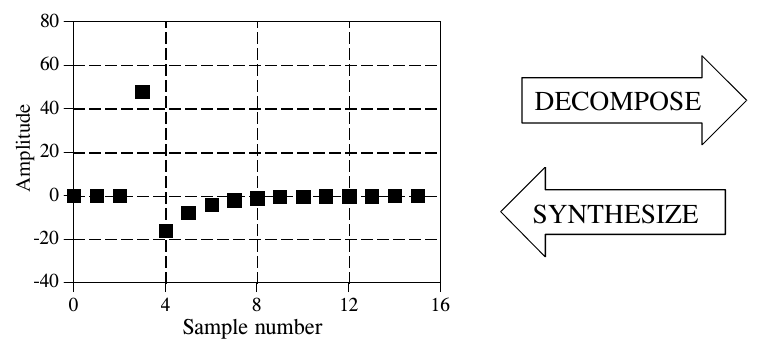
\includegraphics[width=0.633\linewidth,height=0.8\textheight,keepaspectratio]{assets/ch08/fig8-01a.png}
\caption*{\textbf{图 8-1a　一个 16 点的示例信号。}（对应的分解见下一张图 8-1b。）
（Amplitude = 幅度，Sample number = 采样序号，DECOMPOSE =
分解，SYNTHESIZE = 合成。）}
\end{figure}

\begin{figure}[htbp]
\centering
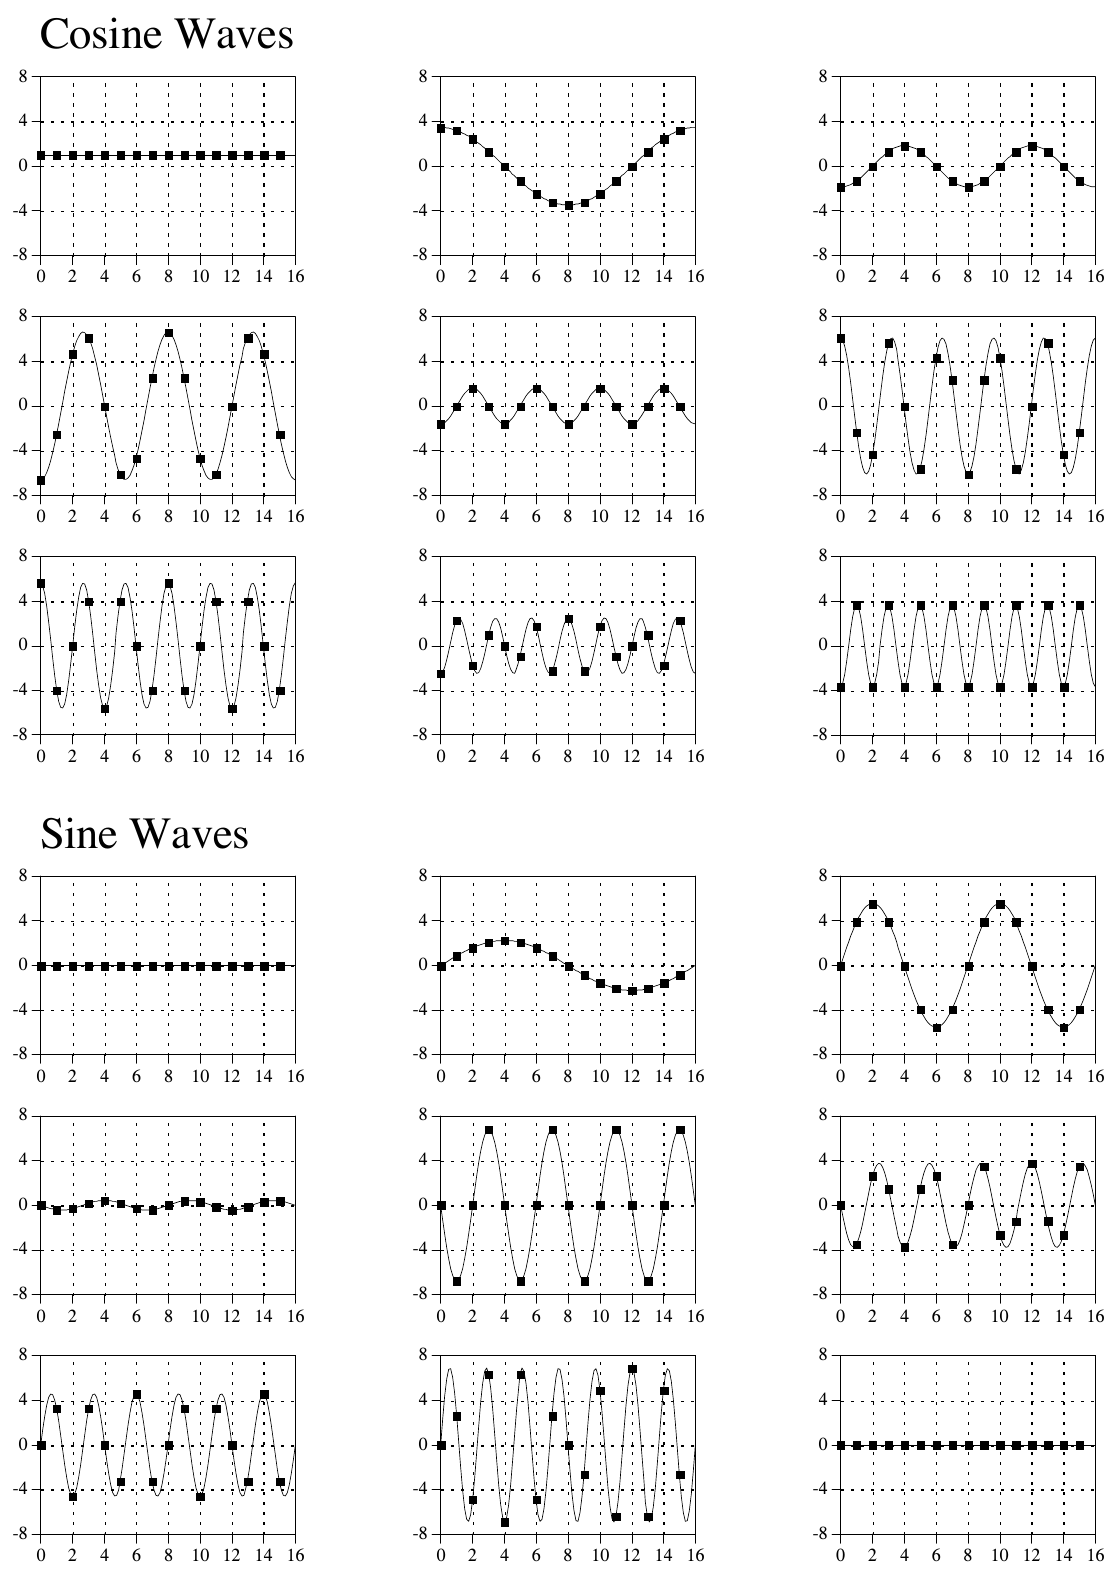
\includegraphics[width=0.925\linewidth,height=0.8\textheight,keepaspectratio]{assets/ch08/fig8-01b.png}
\caption*{\textbf{图 8-1b　傅里叶分解的例子。} 一个 16 点的信号（图 8-1a）被分解成
9 个余弦波和 9
个正弦波。每个正弦波的频率是固定的，只有幅度会随被分解的波形而变。
（Cosine Waves = 余弦波，Sine Waves =
正弦波。每组九幅图按从左到右、从上到下的顺序，频率依次为 0～8，即在 16
个点里走完 0～8 个周期。）}
\end{figure}

为什么用正弦波，而不用比如方波或三角波？记住，分解一个信号的方法有无穷多种。分解的目的，是得到一些比原信号更容易处理的东西。例如，冲激分解让我们可以一次考察信号的一个点，由此得到了卷积这一强大的方法。分量正弦波和余弦波比原信号简单，是因为它们具有一个原信号没有的性质：正弦保真性(sinusoidal
fidelity)。第 5
章讲过，正弦波输入一个系统，保证得到的输出也是正弦波。只有信号的幅度和相位可以改变，频率和波形必须保持不变。正弦波是唯一具有这一有用性质的波形。方波或三角波分解虽然也做得到，但一般没有理由说它们有用。

傅里叶变换(Fourier
transform)这个总称可以分成四类，对应可能遇到的四种基本信号类型。一个信号可以是连续的或离散的，也可以是周期的或非周期的。这两个特征组合起来就得到四类，下面分别说明，并画在图
8-2 中。

\textbf{非周期---连续(Aperiodic-Continuous)}
例如衰减指数函数和高斯曲线。这类信号向正负无穷两个方向延伸，不按周期模式重复。用于这类信号的傅里叶变换就叫傅里叶变换(Fourier
Transform)。

\textbf{周期---连续(Periodic-Continuous)}
例子有：正弦波、方波，以及任何从负无穷到正无穷按固定模式重复的波形。这一版本的傅里叶变换叫傅里叶级数(Fourier
Series)。

\textbf{非周期---离散(Aperiodic-Discrete)}
这类信号只在正负无穷之间的离散点上有定义，并且不按周期重复。这类傅里叶变换叫离散时间傅里叶变换(Discrete
Time Fourier Transform，DTFT)。

\textbf{周期---离散(Periodic-Discrete)}
这是从负无穷到正无穷周期重复的离散信号。这一类傅里叶变换有时叫离散傅里叶级数(Discrete
Fourier Series)，但最常用的名字是离散傅里叶变换(Discrete Fourier
Transform)。

你可能会觉得，这四种傅里叶变换的名字既混乱又没条理。你说得对，这些名字是在
200
年里相当随意地演变出来的。你没有别的办法，只能把它们记住，然后继续往下学。

这四类信号都向正负无穷延伸。等一等，你会说！如果计算机里只存了有限个采样，比如一个
1024
点的信号，怎么办？难道没有一种适用于有限长信号的傅里叶变换吗？没有。正弦波和余弦波的定义就是从负无穷延伸到正无穷。你没法用一组无限长的信号去合成一个有限长的东西。绕过这个难题的办法，是让有限长的数据看起来像一个无限长的信号。做法是想象在实际数据点的左右两边还有无穷多个采样。如果这些''想象出来''的采样全为零，信号看起来就是离散、非周期的，适用离散时间傅里叶变换。另一种做法是让想象出来的采样都是这
1024 个实际点的复制。这时信号看起来是离散、周期的，周期为 1024
个采样，于是就要用离散傅里叶变换。

结果是，合成一个非周期信号需要无穷多个正弦波。这使得离散时间傅里叶变换不可能用计算机算法算出来。排除之后，DSP
中唯一能用的傅里叶变换就是
DFT。换句话说，数字计算机只能处理离散、有限长的信息。当你钻研理论问题、对付习题、琢磨数学谜题时，可能会用到傅里叶变换家族的前三个成员。当你坐到计算机前，你只会用
DFT。后面的章节会简要介绍其他几种傅里叶变换。眼下，请集中精力理解离散傅里叶变换。

\begin{figure}[htbp]
\centering
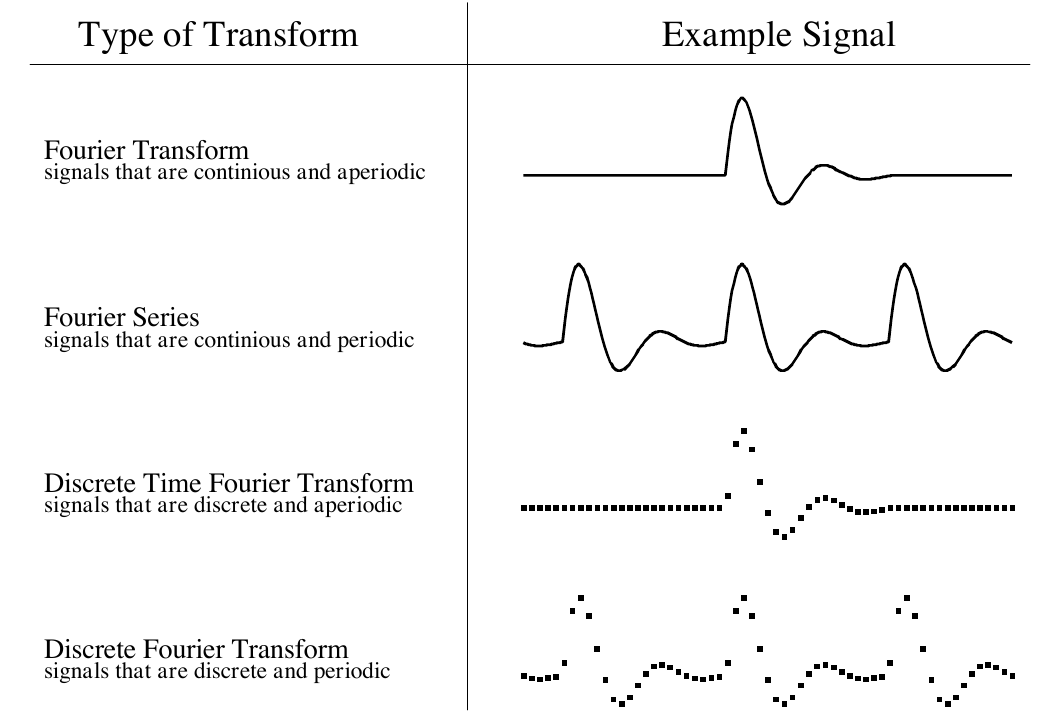
\includegraphics[width=0.875\linewidth,height=0.8\textheight,keepaspectratio]{assets/ch08/fig8-02.png}
\caption*{\textbf{图 8-2　四种傅里叶变换的示意图。}
信号可以是连续的或离散的，也可以是周期的或非周期的。两两组合得到四种可能，每种都有自己版本的傅里叶变换。这些名字没什么条理，直接记住就好。
（Type of Transform = 变换类型，Example Signal = 示例信号；Fourier
Transform：signals that are continuous and aperiodic =
傅里叶变换：连续且非周期的信号；Fourier Series：continuous and periodic
= 傅里叶级数：连续且周期；Discrete Time Fourier Transform：discrete and
aperiodic = 离散时间傅里叶变换：离散且非周期；Discrete Fourier
Transform：discrete and periodic = 离散傅里叶变换：离散且周期。图中
continuous 原书误拼为 continious。）}
\end{figure}

回头看图 8-1 中的 DFT 分解示例。表面上看，这是一个 16 点信号被分解成 18
个正弦波，每个正弦波各有 16 个点。用更正式的说法，(a) 中的 16
点信号必须看作一个无限长周期信号的一个周期。同样，(b) 中的 18
个正弦波，每个都代表一个无限长正弦波中的一段 16 点。把这看作''用 16
点的正弦波合成一个 16
点信号''，还是''用无限长的正弦波合成一个无限长的周期信号''，这真的有关系吗？答案是：通常没关系，但有时有关系。后面的章节会遇到一些
DFT
的性质，如果把信号看作有限长，它们会显得莫名其妙；一旦考虑到周期性，就一目了然了。要理解的关键点是：引入这种周期性，是为了能使用一个数学工具，即
DFT。就信号从哪里来、怎样采集而言，这种周期性通常没有任何意义。

四种傅里叶变换各自都可以再分成实数版本和复数版本。实数版本最简单，合成与分解只用普通的数和代数。例如，图
8-1 就是一个实数 DFT
的例子。四种傅里叶变换的复数版本要复杂得多，需要用到复数。复数是像
\(3 + 4j\) 这样的数，其中 \(j\) 等于 \(\sqrt{-1}\)（电气工程师用变量
j，数学家用变量 i）。复数数学很快就会让人吃不消，即使是专门做 DSP
的人也一样。事实上，本书的一个主要目标就是不用复数数学来讲解 DSP
的基础，让更多的科学家和工程师能看懂。复数傅里叶变换是那些专攻
DSP、并且愿意在数学沼泽里没到脖子的人的领地。如果你有这个兴趣，第 30～33
章会带你去那里。

变换(transform)这个数学术语在数字信号处理中用得非常多，比如：傅里叶变换、拉普拉斯变换(Laplace
transform)、Z 变换(Z transform)、希尔伯特变换(Hilbert
transform)、离散余弦变换(Discrete Cosine
transform)等等。变换到底是什么？要回答这个问题，先回想一下函数是什么。函数是把一个值变成另一个值的算法或过程。例如，\(y = 2x + 1\)
就是一个函数。你给 x 选一个值，代进方程，就会得到一个 y
值。函数也可以把几个值变成一个值，例如 \(y = 2a + 3b + 4c\)，它把
a、b、c 变成 y。

变换是函数的直接推广，它允许输入和输出都有多个值。假设你有一个由 100
个采样组成的信号。如果你设计出某个方程、算法或过程，能把这 100
个采样变成另外 100
个采样，你就有了一个变换。如果你觉得它够有用，你完全有权利把自己的姓冠在它前面，向同事们宣扬它的好处。（如果你是一位杰出的
18
世纪法国数学家，这招效果最好。）变换不限定数据的类型或数量。例如，输入可以是
100 个离散采样，输出可以是 200
个离散采样。同样，输入可以是连续信号，输出也是连续信号。混合的也行：离散输入、连续输出，或者反过来。简单地说，变换就是把一块数据变成另一块数据的任何固定过程。我们来看看这怎样用到眼下的主题：离散傅里叶变换。

\section{实数 DFT 的记号与格式}

如图 8-3 所示，离散傅里叶变换把一个 N 点的输入信号变成两个 N/2+1
点的输出信号。输入信号包含被分解的信号，两个输出信号包含各分量正弦波和余弦波的幅度（按一种稍后讨论的方式做了缩放）。输入信号被称为处在时域(time
domain)。这是因为进入 DFT
的信号最常见的是按固定时间间隔采集的采样。当然，任何采样数据都可以送进
DFT，不管它是怎样采集的。在傅里叶分析中看到''时域''这个词，它可能确实指随时间采集的采样，也可能只是泛指任何正在被分解的离散信号。频域(frequency
domain)这个词用来描述正弦波和余弦波的幅度（包括我们答应要解释的那种特殊缩放）。

\begin{figure}[htbp]
\centering
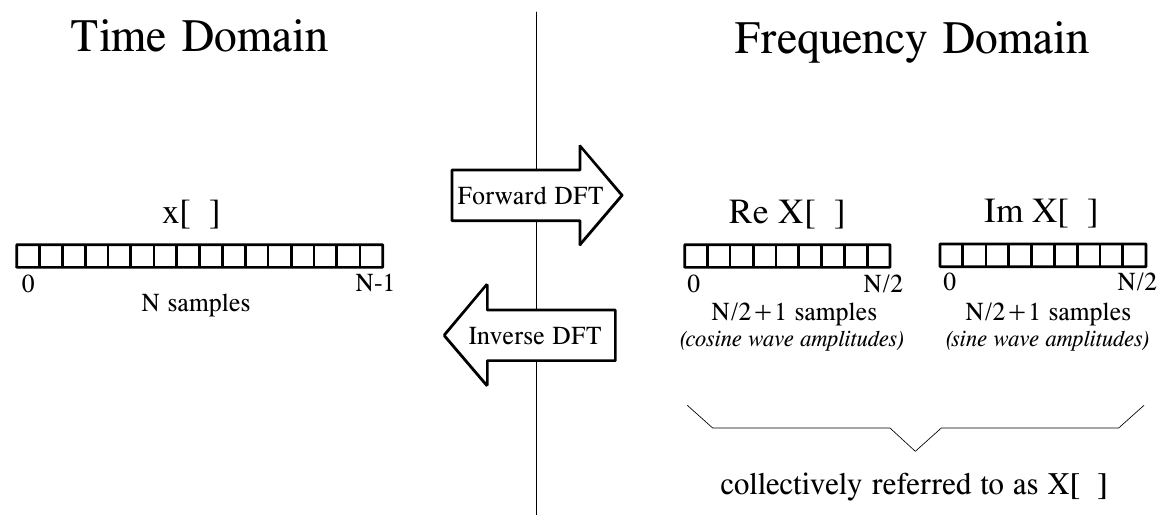
\includegraphics[width=0.975\linewidth,height=0.8\textheight,keepaspectratio]{assets/ch08/fig8-03.png}
\caption*{\textbf{图 8-3　DFT 的术语。} 在时域中，x{[} {]} 由 N 个点组成，序号从 0
到 N−1。在频域中，DFT 产生两个信号：实部(real part)，记作 Re X{[}
{]}；虚部(imaginary part)，记作 Im X{[} {]}。这两个频域信号各长 N/2+1
点，序号从 0 到 N/2。正向 DFT(Forward DFT)把时域变换到频域，逆
DFT(Inverse DFT)把频域变换回时域。（注意：本图描述的是实数 DFT。第 31
章讨论的复数 DFT 是把 N 个复数点变成另一组 N 个复数点。） （Time Domain
= 时域，Frequency Domain = 频域，N samples = N 个采样，N/2+1 samples =
N/2+1 个采样，cosine wave amplitudes = 余弦波幅度，sine wave amplitudes
= 正弦波幅度，collectively referred to as X{[} {]} = 合起来称为 X{[}
{]}。）}
\end{figure}

频域包含的信息和时域完全一样，只是形式不同。知道其中一个域，就能算出另一个。已知时域信号，计算频域的过程叫分解(decomposition)、分析(analysis)、正向
DFT(forward DFT)，或者干脆叫
DFT。已知频域，计算时域的过程叫合成(synthesis)，或逆 DFT(inverse
DFT)。合成与分析都可以写成方程，也都可以写成计算机算法。

时域中的采样数通常用变量 N 表示。N 可以是任何正整数，但通常选 2
的幂，比如 128、256、512、1024
等。原因有两个。第一，数字存储用二进制寻址，2
的幂是很自然的信号长度。第二，计算 DFT
最高效的算法------快速傅里叶变换(Fast Fourier
Transform，FFT)------通常要求 N 是 2 的幂。N 一般在 32 到 4096
之间。多数情况下，采样序号从 0 到 N−1，而不是从 1 到 N。

标准的 DSP 记法用小写字母表示时域信号，比如 x{[} {]}、y{[} {]}、z{[}
{]}。对应的大写字母表示它们的频域，即 X{[} {]}、Y{[} {]}、Z{[}
{]}。举例来说，假设一个 N 点的时域信号存放在 x{[} {]}
中。这个信号的频域叫 X{[} {]}，由两部分组成，每部分是一个 N/2+1
个采样的数组。它们叫 X{[} {]} 的实部，记作 Re X{[} {]}；以及 X{[} {]}
的虚部，记作 Im X{[} {]}。Re X{[} {]} 中的值是余弦波的幅度，Im X{[} {]}
中的值是正弦波的幅度（暂时不管缩放因子）。就像时域从 x{[}0{]} 到
x{[}N−1{]}，频域信号从 Re X{[}0{]} 到 Re X{[}N/2{]}、从 Im X{[}0{]} 到
Im X{[}N/2{]}。仔细研究这些记法，它们对理解 DSP
中的公式至关重要。可惜有些计算机语言不区分大小写，变量名只好由每个程序员自己定。本书的程序用数组
XX{[} {]} 存放时域信号，用数组 REX{[} {]} 和 IMX{[} {]} 存放频域信号。

实部和虚部这两个名字来自复数 DFT，在那里用来区分实数和虚数。实数 DFT
用不着这么复杂的东西。在学到第 31
章之前，只要把''实部''理解成余弦波的幅度、``虚部''理解成正弦波的幅度就行。别被这两个有暗示性的名字误导，这里用到的全是普通的数。

同样，也别被频域信号的长度误导。DSP 文献里常常看到这样的说法：``DFT 把 N
点的时域信号变成 N 点的频域信号。''这指的是复数
DFT，其中每个''点''都是一个复数（由实部和虚部组成）。现在先专心学实数
DFT，难的数学很快就会来。

\section{频域的自变量}

图 8-4 是一个 N = 128 的 DFT 示例。时域信号存放在数组 x{[}0{]} 到
x{[}127{]} 中。频域信号存放在两个数组 Re X{[}0{]} 到 Re X{[}64{]} 和 Im
X{[}0{]} 到 Im X{[}64{]} 中。注意，时域的 128 个点对应每个频域信号的 65
个点，频率序号从 0 到 64。也就是说，时域的 N 个点对应频域的 N/2+1
个点（不是 N/2 个点）。忘掉这个多出来的点，是 DFT 程序中的常见错误。

\begin{figure}[htbp]
\centering
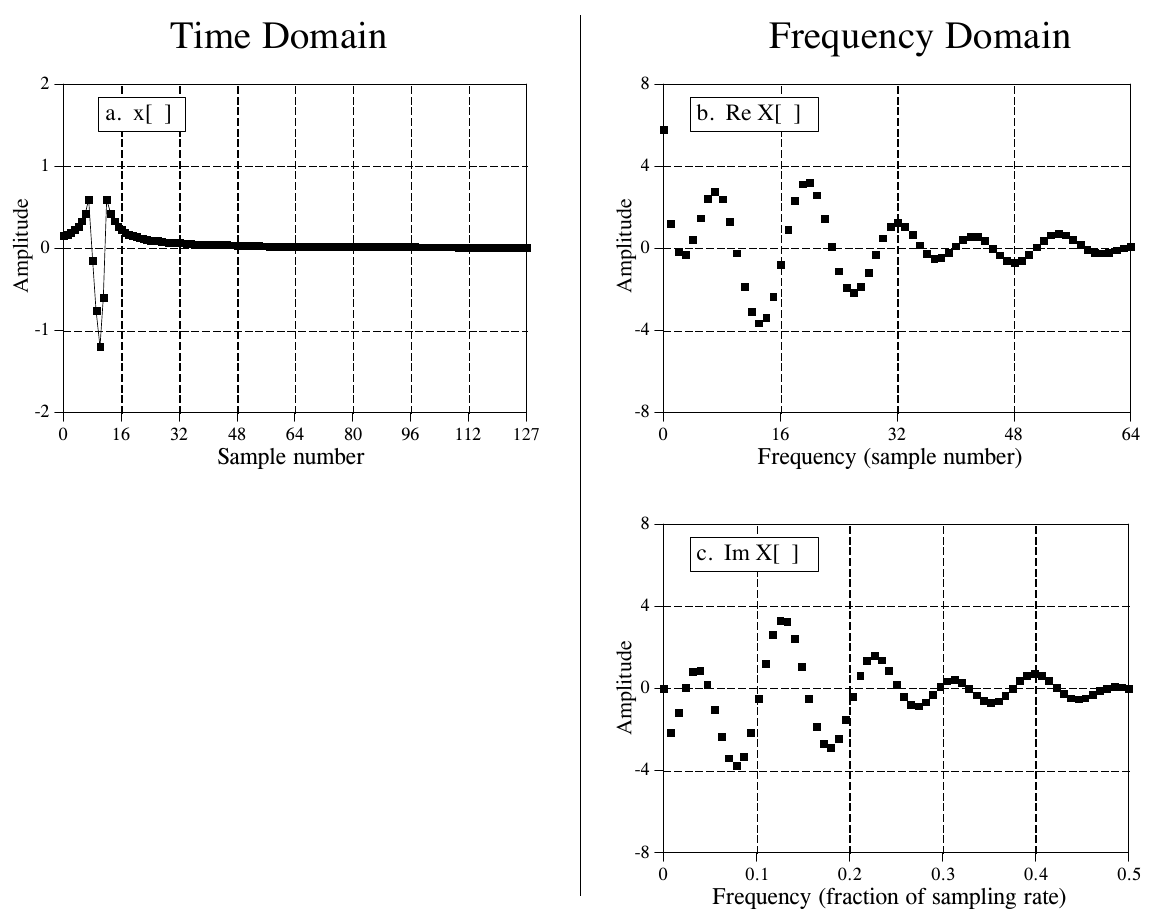
\includegraphics[width=0.958\linewidth,height=0.8\textheight,keepaspectratio]{assets/ch08/fig8-04.png}
\caption*{\textbf{图 8-4　DFT 的例子。} DFT 把时域信号 x{[} {]} 变换成频域信号 Re
X{[} {]} 和 Im X{[} {]}。频域的横轴可以用三种方式之一来标注：(1)
用数组下标，从 0 到 N/2；(2) 用采样频率的分数，从 0 到 0.5；(3)
用自然频率，从 0 到 π。本例中 (b) 用的是第一种方式，(c)
用的是第二种方式。 （Time Domain = 时域，Frequency Domain =
频域，Amplitude = 幅度，Sample number = 采样序号，Frequency (sample
number) = 频率（采样序号），Frequency (fraction of sampling rate) =
频率（采样率的分数）。译注：图注说''三种方式''，正文讲的是四种，第四种是用具体的模拟频率（赫兹）标注，图注没有列出。）}
\end{figure}

频域的横轴有四种不同的标注方式，在 DSP
中都很常见。第一种方式是把横轴标成 0 到 64，对应数组中的第 0 到第 N/2
个采样。用这种标注时，频域的下标是整数，例如 Re X{[}k{]} 和 Im
X{[}k{]}，其中 k 从 0 到 N/2，步长为
1。程序员喜欢这种方式，因为他们写代码就是这样，用一个下标访问数组元素。图
8-4b 用的就是这种记法。

第二种方式用在图 (c) 中，横轴标成采样率的分数。这意味着横轴上的值总是在
0 到 0.5
之间，因为离散数据只能包含从直流(DC)到采样率一半之间的频率。这种记法用的下标是
f，表示频率(frequency)。实部和虚部写成 Re X{[}f{]} 和 Im X{[}f{]}，其中
f 取 0 到 0.5 之间等间距的 N/2+1 个值。要从第一种记法 k 换成第二种记法
f，把横轴除以 N 即可，也就是
\(f = k/N\)。本书大多数图都用第二种方式，以强调离散信号只包含 0 到采样率
0.5 倍之间的频率。

第三种方式和第二种类似，只是横轴乘以 2π。这种标注用的下标是
ω，即小写的希腊字母 omega。在这种记法中，实部和虚部写成 Re X{[}ω{]} 和
Im X{[}ω{]}，其中 ω 取 0 到 π 之间等间距的 N/2+1 个值。参数 ω
叫自然频率(natural frequency)，单位是弧度(radians)。这是基于一个圆有 2π
弧度的想法。数学家喜欢这种方式，因为它让方程更短。例如，看看余弦波在前三种记法中各怎么写：用
k，\(c[n] = \cos(2\pi kn/N)\)；用 f，\(c[n] = \cos(2\pi fn)\)；用
ω，\(c[n] = \cos(\omega n)\)。

第四种方式是按具体应用中用到的模拟频率来标注横轴。例如，如果所研究的系统采样率是
10 kHz（即每秒 10,000 个采样），频域的图就从 0 画到 5
kHz。这种方式的优点是用真实世界的含义来呈现频率数据。缺点是它绑定了一个特定的采样率，因此不适用于一般的
DSP 算法开发，比如数字滤波器设计。

这四种记法在 DSP
中都有人用，你需要习惯在它们之间转换，图和数学公式都包括在内。要判断用的是哪种记法，看自变量和它的取值范围。你应该会看到以下四种之一：k（或别的整数下标），从
0 到 N/2；f，从 0 到 0.5；ω，从 0 到
π；或者用赫兹表示的频率，从直流到实际采样率的一半。

\section{DFT 的基函数}

DFT 中用到的正弦波和余弦波通常叫 DFT 的基函数(basis
functions)。换句话说，DFT 的输出是一组表示幅度的数，基函数则是一组幅度为
1
的正弦波和余弦波。如果把每个幅度（频域）分配给相应的正弦或余弦波（基函数），得到的就是一组经过缩放的正弦波和余弦波，把它们加起来就构成时域信号。

DFT 的基函数由下面的公式生成：

\textbf{公式 8-1　DFT 基函数的公式。} 式中 \(c_k[i]\) 和 \(s_k[i]\)
分别是余弦波和正弦波，每个长 N 点，i 从 0 到 N−1。参数 k
决定波的频率。在 N 点 DFT 中，k 取 0 到 N/2 之间的值。

\[
c_k[i] = \cos(2\pi k i / N)
\]

\[
s_k[i] = \sin(2\pi k i / N)
\]

其中 \(c_k[\,]\) 是与 Re X{[}k{]} 中的幅度对应的余弦波，\(s_k[\,]\) 是与
Im X{[}k{]} 中的幅度对应的正弦波。例如，图 8-5 画出了 N = 32 点 DFT
所用的 17 个正弦波和 17
个余弦波中的一部分。由于这些正弦波要相加构成输入信号，它们必须和输入信号一样长。本例中，每个都有
32 个点，i 从 0 到 31。参数 k
决定每个正弦波的频率。具体来说，\(c_1[\,]\) 是在 N
个点里走完一个完整周期的余弦波，\(c_5[\,]\) 是在 N
个点里走完五个完整周期的余弦波，依此类推。这是理解基函数的一个重要概念：频率参数
k 等于在信号的 N 个点里完成的完整周期数。

\begin{figure}[htbp]
\centering
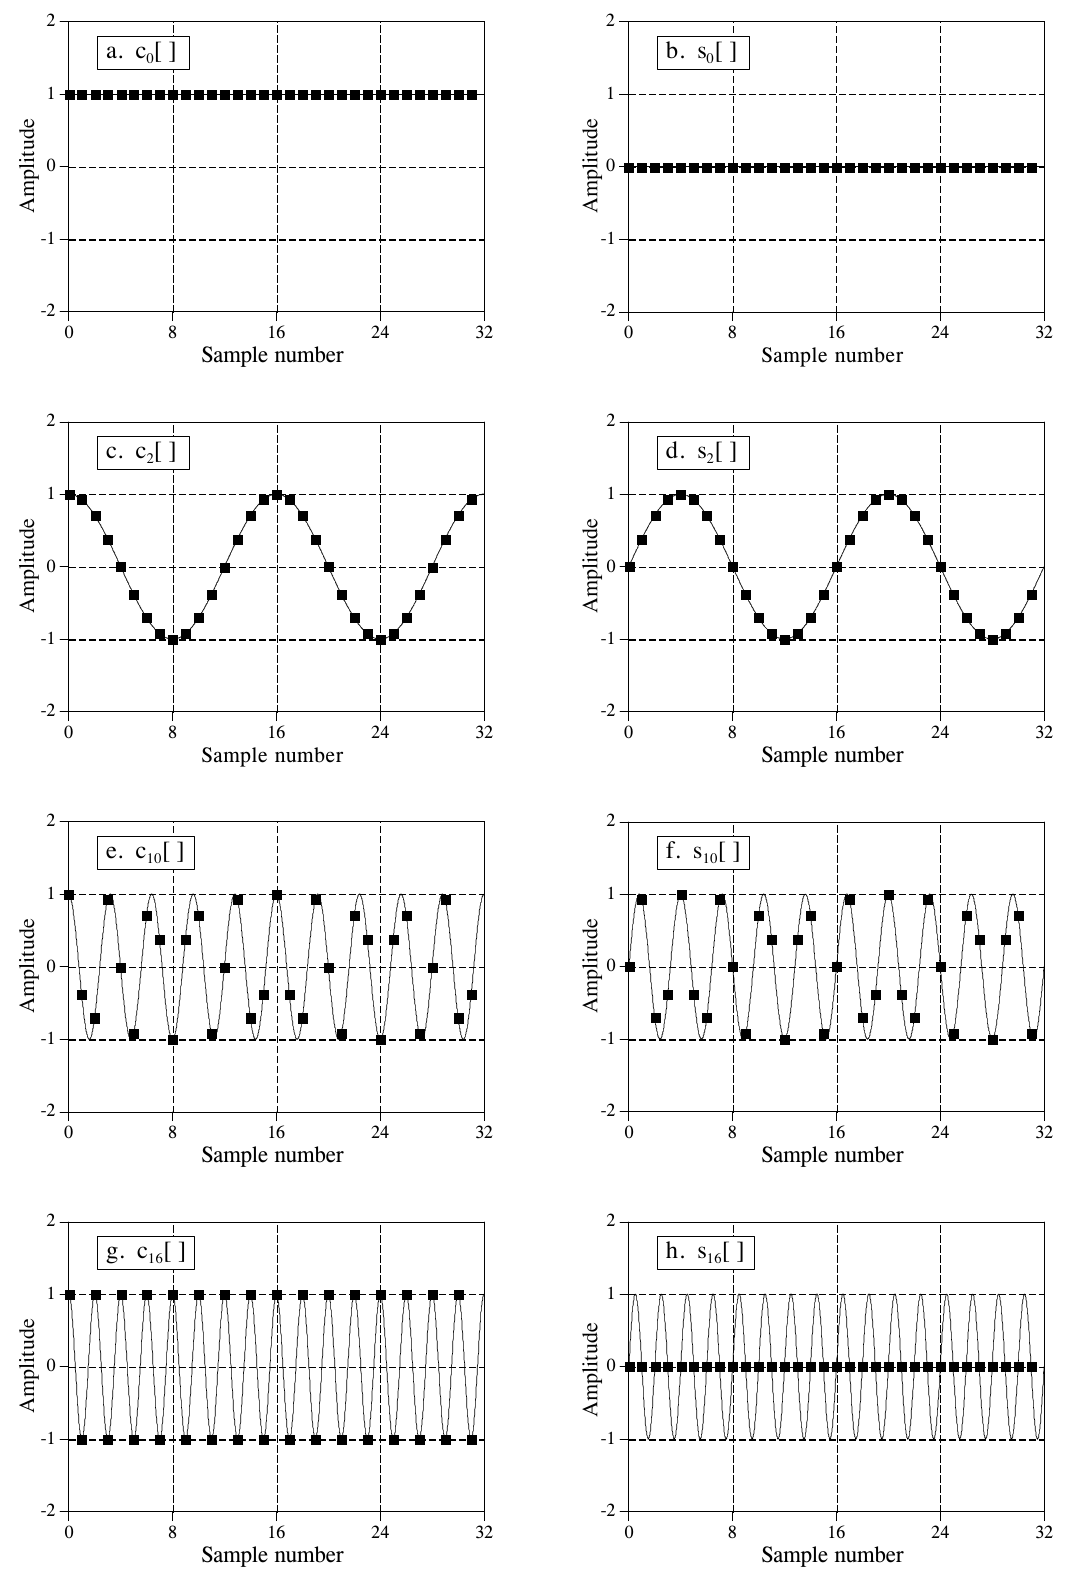
\includegraphics[width=0.892\linewidth,height=0.8\textheight,keepaspectratio]{assets/ch08/fig8-05.png}
\caption*{\textbf{图 8-5　DFT 的基函数。} 32 点 DFT 的基函数有 17 个离散余弦波和
17 个离散正弦波，本图画出其中 8
个。这些都是离散信号；图中的连续曲线只是为了帮助读者的眼睛跟上波形。
（Amplitude = 幅度，Sample number = 采样序号；a～h 分别为
\(c_0\)、\(s_0\)、\(c_2\)、\(s_2\)、\(c_{10}\)、\(s_{10}\)、\(c_{16}\)、\(s_{16}\)。）}
\end{figure}

我们来仔细看几个基函数。图 (a) 是余弦波
\(c_0[\,]\)。这是频率为零的余弦波，是恒为 1 的常数。这意味着 Re X{[}0{]}
存放的是时域信号所有点的平均值。在电子学里会说，Re X{[}0{]}
存放的是直流偏置(DC offset)。频率为零的正弦波 \(s_0[\,]\) 画在 (b)
中，是一个全为零的信号。由于它对合成的时域信号没有任何影响，Im X{[}0{]}
的值无关紧要，总是设为零。稍后还会细说。

图 (c) 和 (d) 是 \(c_2[\,]\) 和 \(s_2[\,]\)，即在 N
个点里完成两个周期的正弦波，分别对应 Re X{[}2{]} 和 Im
X{[}2{]}。同样，(e) 和 (f) 是 \(c_{10}[\,]\) 和 \(s_{10}[\,]\)，即在 N
个点里完成十个周期的正弦波，对应数组 Re X{[}10{]} 和 Im X{[}10{]}
中的幅度。问题是，(e) 和 (f)
中的采样看起来已经不像正弦波和余弦波了。如果图中没有那些连续曲线，你甚至很难看出波形的规律。这也许会让你有点不安，但不用担心。从数学角度看，这些采样确实构成离散的正弦波，即使你的眼睛跟不上它们的规律。

基函数中最高的频率画在 (g) 和 (h) 中。它们是 \(c_{N/2}[\,]\) 和
\(s_{N/2}[\,]\)，本例中就是 \(c_{16}[\,]\) 和
\(s_{16}[\,]\)。离散余弦波在 1 和 −1
之间交替取值，可以理解为在一个连续正弦波的波峰处采样。相反，离散正弦波全为零，这是在过零点处采样的结果。这使得
Im X{[}N/2{]} 和 Im X{[}0{]}
一样，总是等于零，对时域信号的合成没有影响。

这里有个谜题：如果进入 DFT 的是 N 个采样，出来的是 N+2
个采样，多出来的信息是从哪儿来的？答案是：有两个输出采样不含任何信息，这样其余
N 个采样才能完全独立。你可能已经猜到了，不含信息的两个点是 Im X{[}0{]}
和 Im X{[}N/2{]}，也就是总为零的那两个采样。

\section{合成：计算逆 DFT}

把到目前为止讲的内容合在一起，可以写出合成方程：

\textbf{公式 8-2　合成方程。} 式中 x{[}i{]} 是被合成的信号，下标 i 从 0
到 N−1。\(\mathrm{Re}\,\bar{X}[k]\) 和 \(\mathrm{Im}\,\bar{X}[k]\)
分别存放余弦波和正弦波的幅度，k 从 0 到 N/2。公式 8-3
给出把这个方程变成逆 DFT 所需的归一化。

\[
x[i] = \sum_{k=0}^{N/2} \mathrm{Re}\,\bar{X}[k]\cos(2\pi k i/N) + \sum_{k=0}^{N/2} \mathrm{Im}\,\bar{X}[k]\sin(2\pi k i/N)
\]

用文字说，任何 N 点信号 x{[}i{]}，都可以由 N/2+1 个余弦波和 N/2+1
个正弦波相加得到。余弦波和正弦波的幅度分别存放在数组
\(\mathrm{Re}\,\bar{X}[k]\) 和 \(\mathrm{Im}\,\bar{X}[k]\)
中。（译注：原书这里写成''分别存放在 Im X̄{[}k{]} 和 Re X̄{[}k{]}
中''，顺序颠倒了，余弦对应实部、正弦对应虚部。）合成方程把这些幅度乘以基函数，得到一组经过缩放的正弦波和余弦波。把这些缩放后的正弦波和余弦波相加，就得到时域信号
x{[}i{]}。

在公式 8-2 中，数组叫 \(\mathrm{Re}\,\bar{X}[k]\) 和
\(\mathrm{Im}\,\bar{X}[k]\)，而不是 Re X{[}k{]} 和 Im
X{[}k{]}。这是因为合成所需的幅度（在本节讨论中称为
\(\mathrm{Re}\,\bar{X}[k]\) 和
\(\mathrm{Im}\,\bar{X}[k]\)）和信号的频域（记作 Re X{[}k{]} 和 Im
X{[}k{]}）略有不同。这就是我们前面提到的缩放因子问题。虽然两者之间的转换只是一个简单的归一化，它却是计算机程序中的常见错误。要当心！写成公式，两者的转换是：

\textbf{公式 8-3　正弦波幅度与频域值之间的转换。} 式中
\(\mathrm{Re}\,\bar{X}[k]\) 和 \(\mathrm{Im}\,\bar{X}[k]\)
存放合成所需的余弦波和正弦波幅度，Re X{[}k{]} 和 Im X{[}k{]}
存放频域的实部和虚部。和往常一样，N 是时域信号的点数，k 是从 0 到 N/2
的下标。

\[
\mathrm{Re}\,\bar{X}[k] = \frac{\mathrm{Re}\,X[k]}{N/2}
\qquad
\mathrm{Im}\,\bar{X}[k] = -\frac{\mathrm{Im}\,X[k]}{N/2}
\]

但有两个特殊情况：

\[
\mathrm{Re}\,\bar{X}[0] = \frac{\mathrm{Re}\,X[0]}{N}
\qquad
\mathrm{Re}\,\bar{X}[N/2] = \frac{\mathrm{Re}\,X[N/2]}{N}
\]

假设给你一个频域表示，要你合成对应的时域信号。首先，你必须求出正弦波和余弦波的幅度。换句话说，已知
Im X{[}k{]} 和 Re X{[}k{]}，你必须求出 \(\mathrm{Im}\,\bar{X}[k]\) 和
\(\mathrm{Re}\,\bar{X}[k]\)。公式 8-3
就是这一步的数学形式。在计算机程序里做这件事要三步。第一，把频域中所有值除以
N/2。第二，把所有虚部值变号。第三，把实部的第一个和最后一个采样 Re
X{[}0{]} 和 Re X{[}N/2{]} 再除以二。这样就得到公式 8-2
合成所需的幅度。公式 8-2 和 8-3 合起来定义了逆 DFT。

完整的逆 DFT 见表 8-1 中的计算机程序。合成（公式
8-2）有两种编程写法，两种都列出来了。第一种方法是一次生成一个缩放后的正弦波，把它加到一个累加数组里，这个数组最后就成为时域信号。第二种方法是一次算出时域信号的一个采样，即所有余弦波和正弦波对应采样之和。两种方法得到相同的结果。这两个程序的差别很小，只是合成时把内外两层循环对调了。

\textbf{表 8-1}（注释已译成中文）

\begin{Shaded}
\begin{Highlighting}[]
\NormalTok{100 \textquotesingle{}THE INVERSE DISCRETE FOURIER TRANSFORM}
\NormalTok{110 \textquotesingle{}时域信号 XX[ ] 由频域信号 REX[ ] 和 IMX[ ] 计算得到。}
\NormalTok{120 \textquotesingle{}}
\NormalTok{130 \textquotesingle{}}
\NormalTok{140 DIM XX[511]                      \textquotesingle{}XX[ ] 存放时域信号}
\NormalTok{150 DIM REX[256]                     \textquotesingle{}REX[ ] 存放频域的实部}
\NormalTok{160 DIM IMX[256]                     \textquotesingle{}IMX[ ] 存放频域的虚部}
\NormalTok{170 \textquotesingle{}}
\NormalTok{180 PI = 3.14159265                  \textquotesingle{}设定常数 PI}
\NormalTok{190 N\% = 512                         \textquotesingle{}N\% 是 XX[ ] 的点数}
\NormalTok{200 \textquotesingle{}}
\NormalTok{210 GOSUB XXXX                       \textquotesingle{}虚构的子程序，把数据载入 REX[ ] 和 IMX[ ]}
\NormalTok{220 \textquotesingle{}}
\NormalTok{230}
\NormalTok{240 \textquotesingle{}                                \textquotesingle{}用公式 8{-}3 求出余弦波和正弦波的幅度}
\NormalTok{250 FOR K\% = 0 TO 256}
\NormalTok{260 REX[K\%] = REX[K\%] / (N\%/2)}
\NormalTok{270 IMX[K\%] = {-}IMX[K\%] / (N\%/2)}
\NormalTok{280 NEXT K\%}
\NormalTok{290 \textquotesingle{}}
\NormalTok{300 REX[0] = REX[0] / 2}
\NormalTok{310 REX[256] = REX[256] / 2}
\NormalTok{320 \textquotesingle{}}
\NormalTok{330 \textquotesingle{}}
\NormalTok{340 FOR I\% = 0 TO 511                \textquotesingle{}把 XX[ ] 清零，好当累加器用}
\NormalTok{350 XX[I\%] = 0}
\NormalTok{360 NEXT I\%}
\NormalTok{370 \textquotesingle{}}
\NormalTok{380 \textquotesingle{}                                公式 8{-}2 合成方法 \#1。逐个频率循环，}
\NormalTok{390 \textquotesingle{}                                生成整条正弦波和余弦波，}
\NormalTok{400 \textquotesingle{}                                并把它们加到累加信号 XX[ ] 中}
\NormalTok{410 \textquotesingle{}}
\NormalTok{420 FOR K\% = 0 TO 256                \textquotesingle{}K\% 遍历 REX[ ] 和 IMX[ ] 中的每个采样}
\NormalTok{430 FOR I\% = 0 TO 511                \textquotesingle{}I\% 遍历 XX[ ] 中的每个采样}
\NormalTok{440 \textquotesingle{}}
\NormalTok{450 XX[I\%] = XX[I\%] + REX[K\%] * COS(2*PI*K\%*I\%/N\%)}
\NormalTok{460 XX[I\%] = XX[I\%] + IMX[K\%] * SIN(2*PI*K\%*I\%/N\%)}
\NormalTok{470 \textquotesingle{}}
\NormalTok{480 NEXT I\%}
\NormalTok{490 NEXT K\%}
\NormalTok{500 \textquotesingle{}}
\NormalTok{510 END}
\end{Highlighting}
\end{Shaded}

第 380～510 行的另一种写法：

\begin{Shaded}
\begin{Highlighting}[]
\NormalTok{380 \textquotesingle{}                       公式 8{-}2 合成方法 \#2。逐个时域采样循环，}
\NormalTok{390 \textquotesingle{}                       把每个余弦波和正弦波的对应采样加起来}
\NormalTok{400 \textquotesingle{}}
\NormalTok{410 \textquotesingle{}}
\NormalTok{420 FOR I\% = 0 TO 511       \textquotesingle{}I\% 遍历 XX[ ] 中的每个采样}
\NormalTok{430 FOR K\% = 0 TO 256       \textquotesingle{}K\% 遍历 REX[ ] 和 IMX[ ] 中的每个采样}
\NormalTok{440 \textquotesingle{}}
\NormalTok{450 XX[I\%] = XX[I\%] + REX[K\%] * COS(2*PI*K\%*I\%/N\%)}
\NormalTok{460 XX[I\%] = XX[I\%] + IMX[K\%] * SIN(2*PI*K\%*I\%/N\%)}
\NormalTok{470 \textquotesingle{}}
\NormalTok{480 NEXT K\%}
\NormalTok{490 NEXT I\%}
\NormalTok{500 \textquotesingle{}}
\NormalTok{510 END}
\end{Highlighting}
\end{Shaded}

\textbf{C 实现}（完整可编译版本见
\texttt{c/table8-1\_inverse\_dft.c}。程序载入两组答案已知的频域数据：一组是图
8-6 的 N = 512 版本，实部全为 N，应还原成 x{[}0{]} = N
的冲激；另一组由三个分量合成。两种合成方法都实现了，并互相比对）：

\begin{Shaded}
\begin{Highlighting}[]
\PreprocessorTok{\#define N  }\DecValTok{512}\PreprocessorTok{                  }\CommentTok{/* 190 N\% = 512：时域点数 */}
\PreprocessorTok{\#define NF }\OperatorTok{(}\PreprocessorTok{N }\OperatorTok{/}\PreprocessorTok{ }\DecValTok{2}\PreprocessorTok{ }\OperatorTok{+}\PreprocessorTok{ }\DecValTok{1}\OperatorTok{)}\PreprocessorTok{          }\CommentTok{/* 150～160 DIM REX[256]、IMX[256]：频域 N/2+1 点 */}

\CommentTok{/* 公式 8{-}3：频域值 → 合成用的余弦/正弦幅度（原地修改） */}
\DataTypeTok{static} \DataTypeTok{void}\NormalTok{ to\_amplitudes}\OperatorTok{(}\DataTypeTok{double} \OperatorTok{*}\NormalTok{rex}\OperatorTok{,} \DataTypeTok{double} \OperatorTok{*}\NormalTok{imx}\OperatorTok{)}
\OperatorTok{\{}
    \ControlFlowTok{for} \OperatorTok{(}\DataTypeTok{int}\NormalTok{ k }\OperatorTok{=} \DecValTok{0}\OperatorTok{;}\NormalTok{ k }\OperatorTok{\textless{}}\NormalTok{ NF}\OperatorTok{;}\NormalTok{ k}\OperatorTok{++)} \OperatorTok{\{}          \CommentTok{/* 250～280 */}
\NormalTok{        rex}\OperatorTok{[}\NormalTok{k}\OperatorTok{]} \OperatorTok{=}\NormalTok{ rex}\OperatorTok{[}\NormalTok{k}\OperatorTok{]} \OperatorTok{/} \OperatorTok{(}\NormalTok{N }\OperatorTok{/} \DecValTok{2}\OperatorTok{);}          \CommentTok{/* 260：除以 N/2 */}
\NormalTok{        imx}\OperatorTok{[}\NormalTok{k}\OperatorTok{]} \OperatorTok{=} \OperatorTok{{-}}\NormalTok{imx}\OperatorTok{[}\NormalTok{k}\OperatorTok{]} \OperatorTok{/} \OperatorTok{(}\NormalTok{N }\OperatorTok{/} \DecValTok{2}\OperatorTok{);}         \CommentTok{/* 270：除以 N/2 并变号 */}
    \OperatorTok{\}}
\NormalTok{    rex}\OperatorTok{[}\DecValTok{0}\OperatorTok{]} \OperatorTok{=}\NormalTok{ rex}\OperatorTok{[}\DecValTok{0}\OperatorTok{]} \OperatorTok{/} \DecValTok{2}\OperatorTok{;}                    \CommentTok{/* 300：首尾两点带宽只有一半，再除以 2 */}
\NormalTok{    rex}\OperatorTok{[}\NormalTok{N }\OperatorTok{/} \DecValTok{2}\OperatorTok{]} \OperatorTok{=}\NormalTok{ rex}\OperatorTok{[}\NormalTok{N }\OperatorTok{/} \DecValTok{2}\OperatorTok{]} \OperatorTok{/} \DecValTok{2}\OperatorTok{;}            \CommentTok{/* 310 */}
\OperatorTok{\}}

\CommentTok{/* 合成方法 1：逐个频率，把整条余弦/正弦波加进累加器 */}
\DataTypeTok{static} \DataTypeTok{void}\NormalTok{ synthesize\_method1}\OperatorTok{(}\DataTypeTok{const} \DataTypeTok{double} \OperatorTok{*}\NormalTok{rex}\OperatorTok{,} \DataTypeTok{const} \DataTypeTok{double} \OperatorTok{*}\NormalTok{imx}\OperatorTok{,} \DataTypeTok{double} \OperatorTok{*}\NormalTok{xx}\OperatorTok{)}
\OperatorTok{\{}
    \ControlFlowTok{for} \OperatorTok{(}\DataTypeTok{int}\NormalTok{ i }\OperatorTok{=} \DecValTok{0}\OperatorTok{;}\NormalTok{ i }\OperatorTok{\textless{}}\NormalTok{ N}\OperatorTok{;}\NormalTok{ i}\OperatorTok{++)}             \CommentTok{/* 340～360：累加器清零 */}
\NormalTok{        xx}\OperatorTok{[}\NormalTok{i}\OperatorTok{]} \OperatorTok{=} \FloatTok{0.0}\OperatorTok{;}
    \ControlFlowTok{for} \OperatorTok{(}\DataTypeTok{int}\NormalTok{ k }\OperatorTok{=} \DecValTok{0}\OperatorTok{;}\NormalTok{ k }\OperatorTok{\textless{}}\NormalTok{ NF}\OperatorTok{;}\NormalTok{ k}\OperatorTok{++)}            \CommentTok{/* 420：遍历每个频率 */}
        \ControlFlowTok{for} \OperatorTok{(}\DataTypeTok{int}\NormalTok{ i }\OperatorTok{=} \DecValTok{0}\OperatorTok{;}\NormalTok{ i }\OperatorTok{\textless{}}\NormalTok{ N}\OperatorTok{;}\NormalTok{ i}\OperatorTok{++)} \OperatorTok{\{}       \CommentTok{/* 430：遍历时域每个点 */}
\NormalTok{            xx}\OperatorTok{[}\NormalTok{i}\OperatorTok{]} \OperatorTok{+=}\NormalTok{ rex}\OperatorTok{[}\NormalTok{k}\OperatorTok{]} \OperatorTok{*}\NormalTok{ cos}\OperatorTok{(}\DecValTok{2} \OperatorTok{*}\NormalTok{ PI }\OperatorTok{*}\NormalTok{ k }\OperatorTok{*}\NormalTok{ i }\OperatorTok{/}\NormalTok{ N}\OperatorTok{);}  \CommentTok{/* 450 */}
\NormalTok{            xx}\OperatorTok{[}\NormalTok{i}\OperatorTok{]} \OperatorTok{+=}\NormalTok{ imx}\OperatorTok{[}\NormalTok{k}\OperatorTok{]} \OperatorTok{*}\NormalTok{ sin}\OperatorTok{(}\DecValTok{2} \OperatorTok{*}\NormalTok{ PI }\OperatorTok{*}\NormalTok{ k }\OperatorTok{*}\NormalTok{ i }\OperatorTok{/}\NormalTok{ N}\OperatorTok{);}  \CommentTok{/* 460 */}
        \OperatorTok{\}}
\OperatorTok{\}}

\CommentTok{/* 合成方法 2：逐个时域点，把所有波在这一点的值加起来（内外循环对调） */}
\DataTypeTok{static} \DataTypeTok{void}\NormalTok{ synthesize\_method2}\OperatorTok{(}\DataTypeTok{const} \DataTypeTok{double} \OperatorTok{*}\NormalTok{rex}\OperatorTok{,} \DataTypeTok{const} \DataTypeTok{double} \OperatorTok{*}\NormalTok{imx}\OperatorTok{,} \DataTypeTok{double} \OperatorTok{*}\NormalTok{xx}\OperatorTok{)}
\OperatorTok{\{}
    \ControlFlowTok{for} \OperatorTok{(}\DataTypeTok{int}\NormalTok{ i }\OperatorTok{=} \DecValTok{0}\OperatorTok{;}\NormalTok{ i }\OperatorTok{\textless{}}\NormalTok{ N}\OperatorTok{;}\NormalTok{ i}\OperatorTok{++)} \OperatorTok{\{}           \CommentTok{/* 420：遍历时域每个点 */}
\NormalTok{        xx}\OperatorTok{[}\NormalTok{i}\OperatorTok{]} \OperatorTok{=} \FloatTok{0.0}\OperatorTok{;}
        \ControlFlowTok{for} \OperatorTok{(}\DataTypeTok{int}\NormalTok{ k }\OperatorTok{=} \DecValTok{0}\OperatorTok{;}\NormalTok{ k }\OperatorTok{\textless{}}\NormalTok{ NF}\OperatorTok{;}\NormalTok{ k}\OperatorTok{++)} \OperatorTok{\{}      \CommentTok{/* 430：遍历每个频率 */}
\NormalTok{            xx}\OperatorTok{[}\NormalTok{i}\OperatorTok{]} \OperatorTok{+=}\NormalTok{ rex}\OperatorTok{[}\NormalTok{k}\OperatorTok{]} \OperatorTok{*}\NormalTok{ cos}\OperatorTok{(}\DecValTok{2} \OperatorTok{*}\NormalTok{ PI }\OperatorTok{*}\NormalTok{ k }\OperatorTok{*}\NormalTok{ i }\OperatorTok{/}\NormalTok{ N}\OperatorTok{);}  \CommentTok{/* 450 */}
\NormalTok{            xx}\OperatorTok{[}\NormalTok{i}\OperatorTok{]} \OperatorTok{+=}\NormalTok{ imx}\OperatorTok{[}\NormalTok{k}\OperatorTok{]} \OperatorTok{*}\NormalTok{ sin}\OperatorTok{(}\DecValTok{2} \OperatorTok{*}\NormalTok{ PI }\OperatorTok{*}\NormalTok{ k }\OperatorTok{*}\NormalTok{ i }\OperatorTok{/}\NormalTok{ N}\OperatorTok{);}  \CommentTok{/* 460 */}
        \OperatorTok{\}}
    \OperatorTok{\}}
\OperatorTok{\}}
\end{Highlighting}
\end{Shaded}

运行结果：冲激测试中，x{[}0{]} = 512.000000，其余点与 0 的最大误差约
1e−11；三分量测试与已知答案完全一致。两种合成方法的输出逐点相同。

\begin{figure}[htbp]
\centering
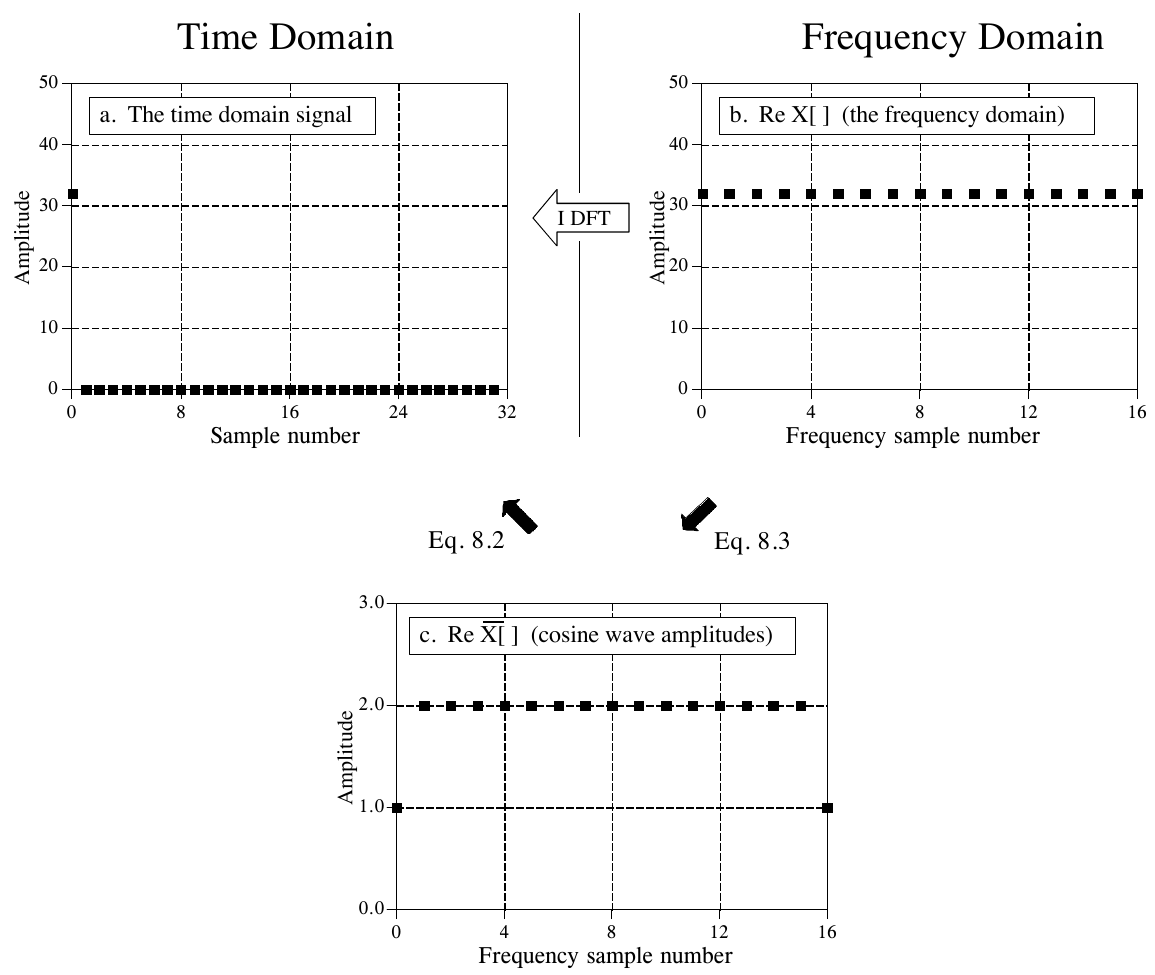
\includegraphics[width=0.963\linewidth,height=0.8\textheight,keepaspectratio]{assets/ch08/fig8-06.png}
\caption*{\textbf{图 8-6　逆 DFT 的例子。} 图 (a) 是一个示例时域信号：位于第 0
个采样、幅度为 32 的冲激。图 (b) 是这个信号频域的实部，是一个值为 32
的常数。频域的虚部（未画出）全为零。图 (c) 是用公式 8-2 重建 (a)
所需的余弦波幅度。(c) 中的值是用公式 8-3 从 (b) 求出来的。 （Time Domain
= 时域，Frequency Domain = 频域，a. The time domain signal = a.
时域信号，b. Re X{[} {]} (the frequency domain) = b. Re X{[}
{]}（频域），c.~Re X̄{[} {]} (cosine wave amplitudes) = c.~Re X̄{[}
{]}（余弦波幅度），I DFT = 逆 DFT，Eq. 8.2 / Eq. 8.3 = 公式 8-2 / 公式
8-3，Sample number = 采样序号，Frequency sample number =
频率采样序号，Amplitude = 幅度。）}
\end{figure}

图 8-6 演示了逆 DFT 的运作，以及频域和合成所需幅度之间的细微差别。图
8-6a 是我们要合成的示例信号：位于第 0 个采样、幅度为 32 的冲激。图 8-6b
是这个信号的频域表示。频域的实部是一个值为 32
的常数，虚部（未画出）全为零。下一章会讲到，这是一个重要的 DFT
变换对：时域中的冲激对应频域中的常数。眼下的要点是：(b) 是 (a) 的
DFT，(a) 是 (b) 的逆 DFT。

公式 8-3 用来把频域信号 (b) 转换成余弦波的幅度
(c)。如图所示，所有余弦波的幅度都是二，只有第 0 和第 16
个采样的值是一。本例没有画出正弦波的幅度，因为它们都为零，没有任何贡献。然后用合成方程（公式
8-2）把余弦波的幅度 (c) 转换成时域信号
(a)。（译注：原书这里写的是''(b)``，应为 (c)。）

这说明了频域和正弦波幅度有什么不同，但没有解释为什么不同。差别的原因在于，频域被定义为一种谱密度(spectral
density)。图 8-7 说明了这是怎么回事。图中的例子是一个 32
点信号频域的实部。和你预期的一样，采样从 0 到 16，代表 0 到采样率 1/2
之间等间距的 17
个频率。谱密度描述的是每单位带宽中有多少信号（幅度）。要把正弦波幅度转换成谱密度，就把每个幅度除以它所代表的带宽。于是引出下一个问题：怎样确定频域中每个离散频率的带宽？

如图所示，可以在采样之间画分界线来确定带宽。例如，第 5 个采样落在 4.5 到
5.5 之间的频带里；第 6 个采样落在 5.5 到 6.5
之间的频带里，依此类推。用总带宽（即 N/2）的分数来表示，每个采样的带宽是
2/N。例外的是两端的采样，它们的带宽只有这个的一半，即
1/N。这就解释了正弦波幅度和频域之间的 2/N
缩放因子，以及首尾两个采样需要额外的因子二。

\begin{figure}[htbp]
\centering
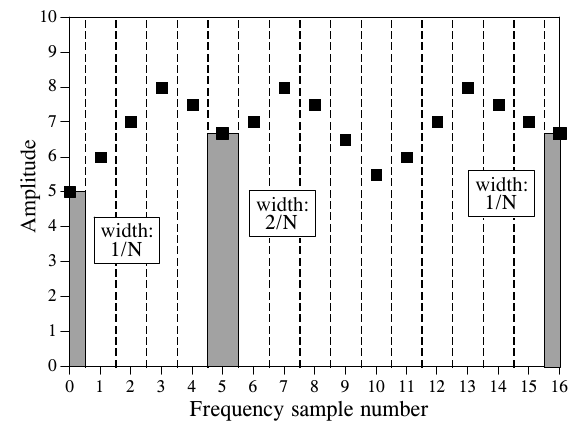
\includegraphics[width=0.483\linewidth,height=0.8\textheight,keepaspectratio]{assets/ch08/fig8-07.png}
\caption*{\textbf{图 8-7　频域采样的带宽。}
频域中的每个采样都可以看作位于一个宽度为 2/N
的频带里（用总带宽的分数表示）。例外的是第一个和最后一个采样，它们的带宽只有一半宽，即
1/N。 （Amplitude = 幅度，Frequency sample number = 频率采样序号，width
= 宽度。）}
\end{figure}

为什么要把虚部变号？这样做只是为了让实数 DFT 和它的老大哥------复数
DFT------保持一致。在第 31 章我们会说明，要让复数 DFT
的数学成立，这样做是必须的。（译注：原书这里写的是''第 29 章''，但第 29
章是《DSP 上手实践》，复数 DFT 在第 31 章，应为笔误。）只处理实数 DFT
时，很多作者不加这个负号。说起来，很多作者连 2/N
这个缩放因子都不加。你要准备好在有些讨论中看到这两样都没有。本书加上它们，有一个极其重要的理由：计算
DFT 最高效的方法是快速傅里叶变换（FFT）算法，第 12 章介绍。FFT
生成的频域就是按公式 8-2 和 8-3
定义的。如果你随意改动这些归一化因子，用到 FFT 的程序就不会按预期工作。

\section{分析：计算 DFT}

DFT
有三种完全不同的计算方法。第一，可以把问题当作一组联立方程来求解。这种方法有助于理解
DFT，但效率太低，没有实用价值。第二种方法借用上一章的一个思想：相关(correlation)。它基于在一个信号中探测一个已知波形。第三种方法叫快速傅里叶变换（FFT），是一种巧妙的算法，它把一个
N 点的 DFT 分解成 N 个各只有一个点的 DFT。FFT
通常比其他方法快几百倍。这里讨论前两种方法，FFT 是第 12
章的主题。重要的是要记住，三种方法的输出完全相同。该用哪一种？实际中，如果
DFT 少于大约 32 点，首选相关法，否则用 FFT。

\subsection{用联立方程求 DFT}

可以这样来思考 DFT 的计算。给你时域中的 N 个值，要你算出频域的 N
个值（不算那两个你知道一定为零的频域值）。初等代数给出了答案：要解出 N
个未知数，必须能写出 N
个线性无关的方程。做法是取每个正弦波的第一个采样并把它们加起来。这个和必须等于时域信号的第一个采样，这就给出了第一个方程。同样，可以对时域信号其余的每个点各写一个方程，得到所需的
N 个方程。然后用解联立方程的成熟方法，比如高斯消元法(Gauss
Elimination)，就能求出解。可惜这种方法需要极大的计算量，在 DSP
中几乎从来不用。但它在另一方面很重要：它说明了为什么能把信号分解成正弦波、需要多少个正弦波，以及基函数必须线性无关（稍后还会细说）。

\subsection{用相关求 DFT}

我们来看一种更好的方法，也是计算 DFT
的标准方法。用一个例子来说明它怎样工作。假设我们要计算一个 64 点信号的
DFT。这意味着要算出频域实部的 33 个点和虚部的 33
个点。本例只说明怎样计算一个采样 Im X{[}3{]}，即在第 0 点到第 63
点之间走完三个完整周期的正弦波的幅度。频域的其他值都用类似的方法计算。

图 8-8 演示了用相关计算 Im X{[}3{]}。图 (a) 和 (b)
是两个示例时域信号，分别叫 x1{[} {]} 和 x2{[} {]}。第一个信号 x1{[} {]}
只由一个在第 0 点到第 63 点之间走三个周期的正弦波组成。相反，x2{[} {]}
由几个正弦波和余弦波组成，没有一个在第 0 点到第 63
点之间走三个周期。这两个信号说明了计算 Im X{[}3{]}
的算法必须做到什么。输入 x1{[} {]} 时，算法必须给出
32，即信号中所含正弦波的幅度（经过公式 8-3
的缩放因子修正）。相比之下，输入另一个信号 x2{[} {]}
时，算法必须给出零，表示这个信号中没有这个特定的正弦波。（译注：按公式
8-4 带负号的定义，x1{[} {]} 实际算出来的 Im X{[}3{]} 是
−32，这里的''32''指幅度大小。本章 C 程序
\texttt{c/table8-2\_dft\_correlation.c} 实测为 −32.000000。）

相关的概念在第 7
章介绍过。回忆一下，要在一个信号中探测一个已知波形，就把两个信号相乘，再把结果信号的所有点加起来。这个过程得到的单个数值，衡量的是两个信号有多相似。图
8-8 演示了这种方法。图 (c) 和 (d) 都画出了我们要找的信号：一个在第 0
和第 63 个采样之间走 3 个周期的正弦波。图 (e) 是 (a) 和 (c)
相乘的结果。同样，(f) 是 (b) 和 (d) 相乘的结果。(e) 中所有点之和是
32，而 (f) 中所有点之和是零，说明我们找到了所需的算法。

\begin{figure}[htbp]
\centering
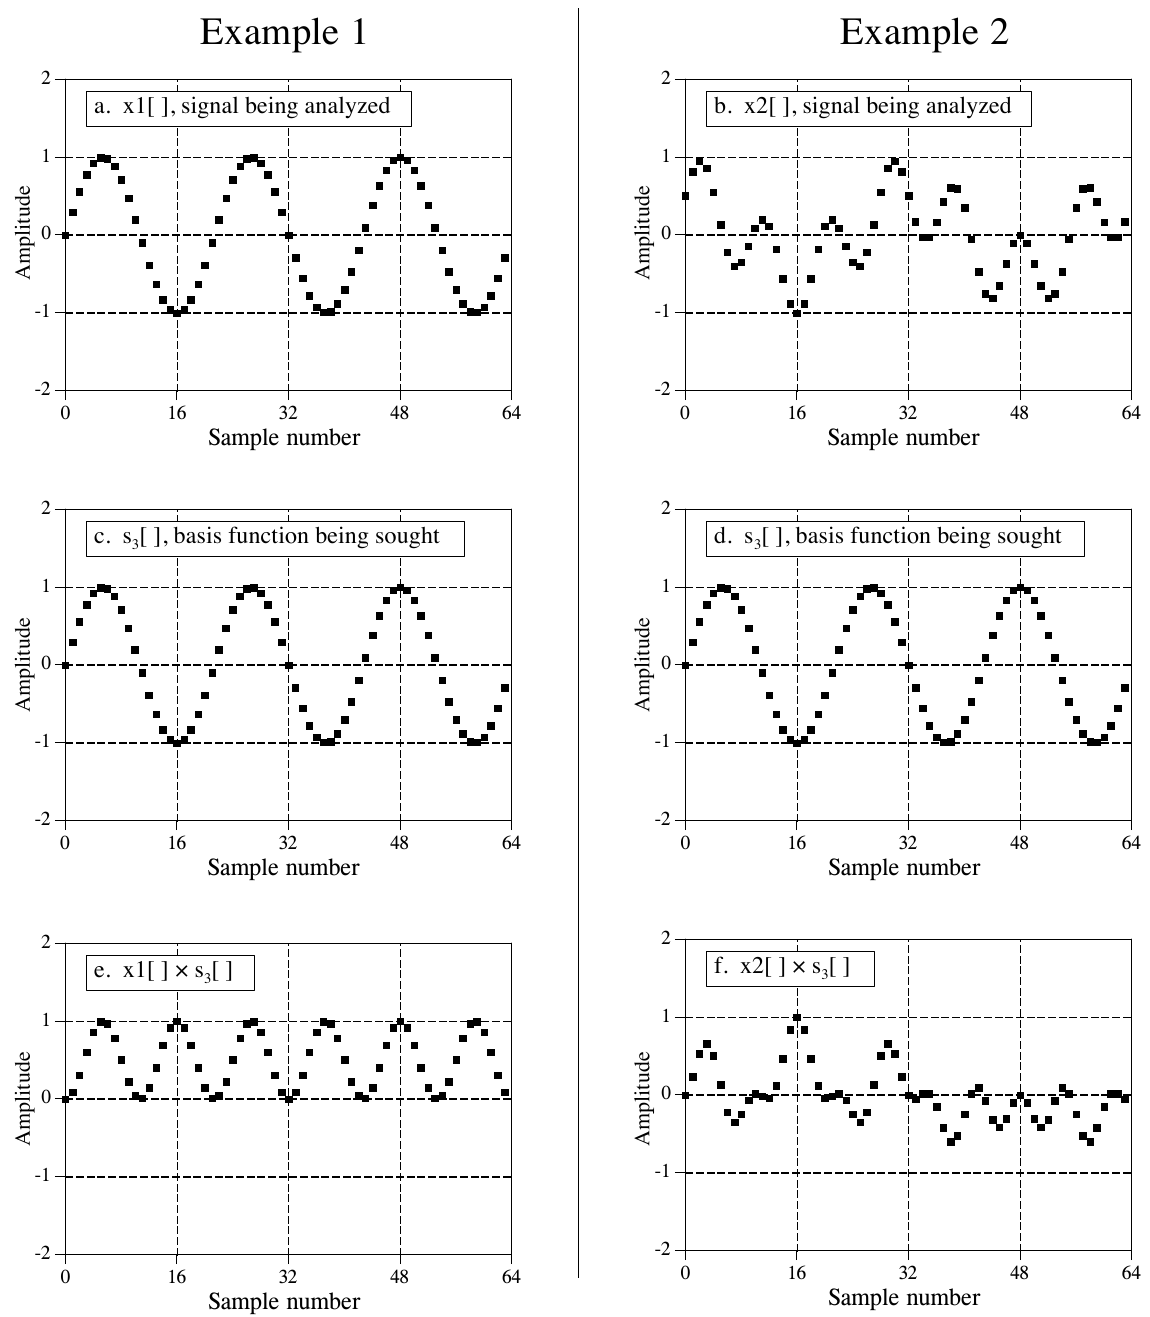
\includegraphics[width=0.958\linewidth,height=0.8\textheight,keepaspectratio]{assets/ch08/fig8-08.png}
\caption*{\textbf{图 8-8　用相关寻找基函数。} 分析两个示例信号 (a) 和
(b)，看它们是否含有 (c) 和 (d) 所示的特定基函数。图 (e) 和 (f)
是每个示例信号与基函数相乘的结果。图 (e) 的平均值为 0.5，说明 x1{[} {]}
含有这个基函数，幅度为 1.0。反过来，(f) 的平均值为零，说明 x2{[} {]}
不含这个基函数。 （Example 1 / Example 2 = 例 1 / 例 2，signal being
analyzed = 被分析的信号，basis function being sought =
要寻找的基函数，Amplitude = 幅度，Sample number = 采样序号。）}
\end{figure}

频域的其他采样用同样的方法计算。这个过程被形式化为分析方程(analysis
equation)，即从时域计算频域的数学方法：

\textbf{公式 8-4　计算 DFT 的分析方程。} 式中 x{[}i{]}
是被分析的时域信号，Re X{[}k{]} 和 Im X{[}k{]} 是要计算的频域信号。下标
i 从 0 到 N−1，下标 k 从 0 到 N/2。

\[
\mathrm{Re}\,X[k] = \sum_{i=0}^{N-1} x[i]\cos(2\pi k i/N)
\]

\[
\mathrm{Im}\,X[k] = -\sum_{i=0}^{N-1} x[i]\sin(2\pi k i/N)
\]

用文字说，频域中的每个采样，都是把时域信号乘以要找的正弦或余弦波，再把结果的各点相加得到的。如果有人问你在做什么，就自信地说：``我在把输入信号和每个基函数做相关。''表
8-2 是用这种方法计算 DFT 的计算机程序。

分析方程不需要像合成方程那样特殊处理首尾两点。不过，公式 8-4
的虚部里有一个负号。和前面一样，这个负号是为了让实数 DFT 和复数 DFT
保持一致，并不是所有书里都有。

要让这个相关算法成立，基函数必须具有一个有意思的性质：每个基函数都必须和其他所有基函数完全不相关。也就是说，任取两个基函数相乘，结果各点之和都等于零。具有这个性质的基函数叫正交的(orthogonal)。（原书误拼为
orthognal。）还有很多别的正交基函数，包括方波、三角波、冲激等。也可以用相关把信号分解到这些别的正交基函数上，就像这里用正弦波做的那样。这并不是说这样做有用，只是说它做得到。

\textbf{表 8-2}（注释已译成中文）

\begin{Shaded}
\begin{Highlighting}[]
\NormalTok{100 \textquotesingle{}THE DISCRETE FOURIER TRANSFORM}
\NormalTok{110 \textquotesingle{}频域信号 REX[ ] 和 IMX[ ] 由时域信号 XX[ ] 计算得到。}
\NormalTok{120 \textquotesingle{}}
\NormalTok{130 \textquotesingle{}}
\NormalTok{140 DIM XX[511]                       \textquotesingle{}XX[ ] 存放时域信号}
\NormalTok{150 DIM REX[256]                      \textquotesingle{}REX[ ] 存放频域的实部}
\NormalTok{160 DIM IMX[256]                      \textquotesingle{}IMX[ ] 存放频域的虚部}
\NormalTok{170 \textquotesingle{}}
\NormalTok{180 PI = 3.14159265                   \textquotesingle{}设定常数 PI}
\NormalTok{190 N\% = 512                          \textquotesingle{}N\% 是 XX[ ] 的点数}
\NormalTok{200 \textquotesingle{}}
\NormalTok{210 GOSUB XXXX                        \textquotesingle{}虚构的子程序，把数据载入 XX[ ]}
\NormalTok{220 \textquotesingle{}}
\NormalTok{230 \textquotesingle{}}
\NormalTok{240 FOR K\% = 0 TO 256                 \textquotesingle{}把 REX[ ] 和 IMX[ ] 清零，好当累加器用}
\NormalTok{250 REX[K\%] = 0}
\NormalTok{260 IMX[K\%] = 0}
\NormalTok{270 NEXT K\%}
\NormalTok{280 \textquotesingle{}}
\NormalTok{290 \textquotesingle{}                                 \textquotesingle{}把 XX[ ] 与余弦波、正弦波做相关，公式 8{-}4}
\NormalTok{300 \textquotesingle{}}
\NormalTok{310 FOR K\% = 0 TO 256                 \textquotesingle{}K\% 遍历 REX[ ] 和 IMX[ ] 中的每个采样}
\NormalTok{320 FOR I\% = 0 TO 511                 \textquotesingle{}I\% 遍历 XX[ ] 中的每个采样}
\NormalTok{330 \textquotesingle{}}
\NormalTok{340 REX[K\%] = REX[K\%] + XX[I\%] * COS(2*PI*K\%*I\%/N\%)}
\NormalTok{350 IMX[K\%] = IMX[K\%] {-} XX[I\%] * SIN(2*PI*K\%*I\%/N\%)}
\NormalTok{360 \textquotesingle{}}
\NormalTok{370 NEXT I\%}
\NormalTok{380 NEXT K\%}
\NormalTok{390 \textquotesingle{}}
\NormalTok{400 END}
\end{Highlighting}
\end{Shaded}

\textbf{C 实现}（完整可编译版本见
\texttt{c/table8-2\_dft\_correlation.c}。程序用书中有答案的例子检验：图
8-6 的冲激、图 8-8 的 x1{[} {]} 和不含 3 周期分量的信号，再把一个 512
点随机信号做 DFT 后用逆 DFT 合成回去）：

\begin{Shaded}
\begin{Highlighting}[]
\CommentTok{/* 相关法 DFT：每个频域点 = 输入信号与对应基函数的相关 */}
\DataTypeTok{static} \DataTypeTok{void}\NormalTok{ dft}\OperatorTok{(}\DataTypeTok{const} \DataTypeTok{double} \OperatorTok{*}\NormalTok{xx}\OperatorTok{,} \DataTypeTok{int}\NormalTok{ n}\OperatorTok{,} \DataTypeTok{double} \OperatorTok{*}\NormalTok{rex}\OperatorTok{,} \DataTypeTok{double} \OperatorTok{*}\NormalTok{imx}\OperatorTok{)}
\OperatorTok{\{}
    \ControlFlowTok{for} \OperatorTok{(}\DataTypeTok{int}\NormalTok{ k }\OperatorTok{=} \DecValTok{0}\OperatorTok{;}\NormalTok{ k }\OperatorTok{\textless{}=}\NormalTok{ n }\OperatorTok{/} \DecValTok{2}\OperatorTok{;}\NormalTok{ k}\OperatorTok{++)} \OperatorTok{\{}     \CommentTok{/* 240～270：REX[] 和 IMX[] 清零，当累加器用 */}
\NormalTok{        rex}\OperatorTok{[}\NormalTok{k}\OperatorTok{]} \OperatorTok{=} \FloatTok{0.0}\OperatorTok{;}
\NormalTok{        imx}\OperatorTok{[}\NormalTok{k}\OperatorTok{]} \OperatorTok{=} \FloatTok{0.0}\OperatorTok{;}
    \OperatorTok{\}}
    \ControlFlowTok{for} \OperatorTok{(}\DataTypeTok{int}\NormalTok{ k }\OperatorTok{=} \DecValTok{0}\OperatorTok{;}\NormalTok{ k }\OperatorTok{\textless{}=}\NormalTok{ n }\OperatorTok{/} \DecValTok{2}\OperatorTok{;}\NormalTok{ k}\OperatorTok{++)}        \CommentTok{/* 310：遍历频域每个点 */}
        \ControlFlowTok{for} \OperatorTok{(}\DataTypeTok{int}\NormalTok{ i }\OperatorTok{=} \DecValTok{0}\OperatorTok{;}\NormalTok{ i }\OperatorTok{\textless{}}\NormalTok{ n}\OperatorTok{;}\NormalTok{ i}\OperatorTok{++)} \OperatorTok{\{}       \CommentTok{/* 320：遍历时域每个点 */}
\NormalTok{            rex}\OperatorTok{[}\NormalTok{k}\OperatorTok{]} \OperatorTok{+=}\NormalTok{ xx}\OperatorTok{[}\NormalTok{i}\OperatorTok{]} \OperatorTok{*}\NormalTok{ cos}\OperatorTok{(}\DecValTok{2} \OperatorTok{*}\NormalTok{ PI }\OperatorTok{*}\NormalTok{ k }\OperatorTok{*}\NormalTok{ i }\OperatorTok{/}\NormalTok{ n}\OperatorTok{);}  \CommentTok{/* 340 */}
\NormalTok{            imx}\OperatorTok{[}\NormalTok{k}\OperatorTok{]} \OperatorTok{{-}=}\NormalTok{ xx}\OperatorTok{[}\NormalTok{i}\OperatorTok{]} \OperatorTok{*}\NormalTok{ sin}\OperatorTok{(}\DecValTok{2} \OperatorTok{*}\NormalTok{ PI }\OperatorTok{*}\NormalTok{ k }\OperatorTok{*}\NormalTok{ i }\OperatorTok{/}\NormalTok{ n}\OperatorTok{);}  \CommentTok{/* 350：注意负号 */}
        \OperatorTok{\}}
\OperatorTok{\}}
\end{Highlighting}
\end{Shaded}

运行结果：图 8-6 的冲激，Re X{[} {]} 全为 32、Im X{[} {]} 全为 0；图 8-8
的 x1{[} {]}，Im X{[}3{]} = −32.000000；不含 3 周期分量的信号，Im
X{[}3{]} \dspsym{≈} 3e−15（即 0）；512 点随机信号做 DFT 再逆
DFT，与原信号的最大误差约 5e−14，Im X{[}0{]} 和 Im X{[}N/2{]} 都为 0。

前面表 8-1 已经说明，逆 DFT
在程序里有两种实现方式，差别在于合成时对调内外两层循环。这不改变程序的输出，但改变你看待这个计算的方式。表
8-2 的 DFT 程序也可以这样改，把第 310～380
行的内外循环对调。和前面一样，程序的输出不变，但思考计算的方式不同。（这两种看待
DFT 和逆 DFT 的方式，可以像卷积那样，称为''输入端''和''输出端''算法。）

按表 8-2
现在的写法，它描述的是频域中的一个采样怎样受时域中所有采样的影响。也就是说，程序依次算出频域中的每个值，而不是一起算。把内外循环对调后，程序就逐个遍历时域中的采样，计算这个点对频域的贡献。整个频域就是把各个时域点的贡献加起来得到的。这引出了下一个问题：时域中的单个采样对频域提供什么样的贡献？答案在傅里叶分析一个有意思的方面里，叫对偶性(duality)。

\section{对偶性}

合成方程和分析方程（公式 8-2 和
8-4）惊人地相似。要从一个域转到另一个域，都是把已知值乘以基函数，再把乘积相加。考虑到我们得出这两个过程的方式完全不同，DFT
和逆 DFT
用的是同一种数学方法，这真是相当了不起。事实上，两个方程唯一的显著差别，源于时域是一个
N 点的信号，而频域是两个 N/2+1 点的信号。后面几章会讲到，复数 DFT
把时域和频域都表示成 N
点的复数信号。这让两个域完全对称，在两者之间转换的方程也几乎一模一样。

时域和频域之间的这种对称叫对偶性，它带来许多有意思的性质。例如，频域中的单个点对应时域中的一个正弦波。由对偶性，反过来也成立：时域中的单个点对应频域中的一个正弦波。再举一个例子，时域中的卷积对应频域中的相乘。由对偶性，反过来也成立：频域中的卷积对应时域中的相乘。第
10 章和第 11 章会更详细地讨论这些以及其他对偶关系。

\section{极坐标表示}

到目前为止，频域被描述为一组余弦波和正弦波的幅度（带一点缩放修正）。这叫直角坐标表示(rectangular
notation)。另一种方式是把频域写成极坐标形式(polar
form)。在这种表示中，Re X{[} {]} 和 Im X{[} {]} 被换成另外两个数组：X{[}
{]} 的幅值(Magnitude)，在公式中写作 Mag X{[} {]}；X{[} {]}
的相位(Phase)，写作 Phase X{[}
{]}。幅值和相位是对实部和虚部的一对一替换。例如，Mag X{[}0{]} 和 Phase
X{[}0{]} 只用 Re X{[}0{]} 和 Im X{[}0{]} 算出。同样，Mag X{[}14{]} 和
Phase X{[}14{]} 只用 Re X{[}14{]} 和 Im X{[}14{]}
算出，依此类推。要理解这种转换，想一想把同一频率的一个余弦波和一个正弦波相加会发生什么。结果是一个同频率的余弦波，但有新的幅度和新的相移(phase
shift)。写成公式，两种表示的关系是：

\textbf{公式 8-5　余弦波与正弦波相加。}
一个余弦波和一个正弦波相加，得到一个幅度和相移都不同的余弦波。A 和 B
中包含的信息被转移到另外两个变量 M 和 θ 中。

\[
A\cos(x) + B\sin(x) = M\cos(x + \theta)
\]

要点是这个过程不丢失任何信息：给定一种表示，就能算出另一种。换句话说，幅度
A 和 B 中包含的信息，同样包含在变量 M 和 θ
中。虽然这个方程涉及的是正弦波和余弦波，但它遵循的转换公式和简单的矢量一样。图
8-9 画出了类比的矢量表示：两个变量 A 和 B 可以看作直角坐标系中的量，而 M
和 θ 是极坐标中的参数。

\begin{figure}[htbp]
\centering
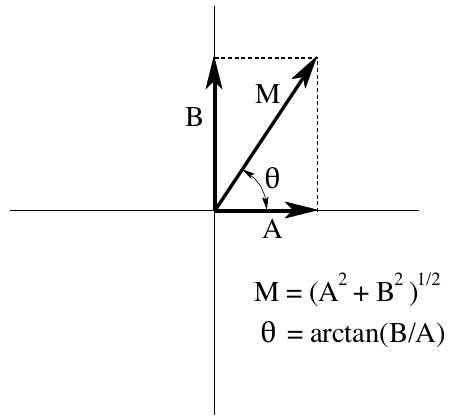
\includegraphics[width=0.383\linewidth,height=0.8\textheight,keepaspectratio]{assets/ch08/fig8-09.png}
\caption*{\textbf{图 8-9　直角坐标到极坐标的转换。}
把一个余弦波和一个（同频率的）正弦波相加，遵循的数学和简单矢量相加一样。
（图中公式：\(M = (A^2 + B^2)^{1/2}\)，\(\theta = \arctan(B/A)\)。）}
\end{figure}

在极坐标表示中，Mag X{[} {]} 存放余弦波的幅度（公式 8-5 和图 8-9 中的
M），Phase X{[} {]} 存放余弦波的相位角（公式 8-5 和图 8-9 中的
θ）。（译注：原书这里两处都写成''公式 8-4''，应为公式
8-5。）下面的公式把频域从直角坐标表示转换成极坐标表示，以及反过来：

\textbf{公式 8-6　直角坐标到极坐标的转换。} 把频域的直角坐标表示 Re
X{[}k{]} 和 Im X{[}k{]} 变成极坐标形式 Mag X{[}k{]} 和 Phase X{[}k{]}。

\[
\mathrm{Mag}\,X[k] = \left(\mathrm{Re}\,X[k]^2 + \mathrm{Im}\,X[k]^2\right)^{1/2}
\]

\[
\mathrm{Phase}\,X[k] = \arctan\!\left(\frac{\mathrm{Im}\,X[k]}{\mathrm{Re}\,X[k]}\right)
\]

\textbf{公式 8-7　极坐标到直角坐标的转换。} 把两个数组 Mag X{[}k{]} 和
Phase X{[}k{]} 转换成 Re X{[}k{]} 和 Im X{[}k{]}。

\[
\mathrm{Re}\,X[k] = \mathrm{Mag}\,X[k]\cos(\mathrm{Phase}\,X[k])
\]

\[
\mathrm{Im}\,X[k] = \mathrm{Mag}\,X[k]\sin(\mathrm{Phase}\,X[k])
\]

直角坐标和极坐标表示让你可以用两种不同的方式看待
DFT。用直角坐标表示，DFT 把一个 N 点信号分解成 N/2+1 个余弦波和 N/2+1
个正弦波，每个都有确定的幅度。用极坐标表示，DFT 把一个 N 点信号分解成
N/2+1
个余弦波，每个都有确定的幅度（叫幅值）和相移。为什么极坐标表示用余弦波而不用正弦波？因为正弦波无法表示信号的直流分量，频率为零的正弦波全是零（见图
8-5 a 和 b）。

虽然极坐标和直角坐标表示包含的信息完全相同，但很多情况下，一种比另一种好用。例如，图
8-10
用直角坐标和极坐标两种形式画出了同一个频域信号。警告：别试图看懂实部和虚部的形状，你的脑袋会爆炸！相比之下，极坐标曲线一目了然：只有大约
0.25 以下的频率存在，相移大致和频率成正比。这是一个低通滤波器(low-pass
filter)的频率响应(frequency response)。

\begin{figure}[htbp]
\centering
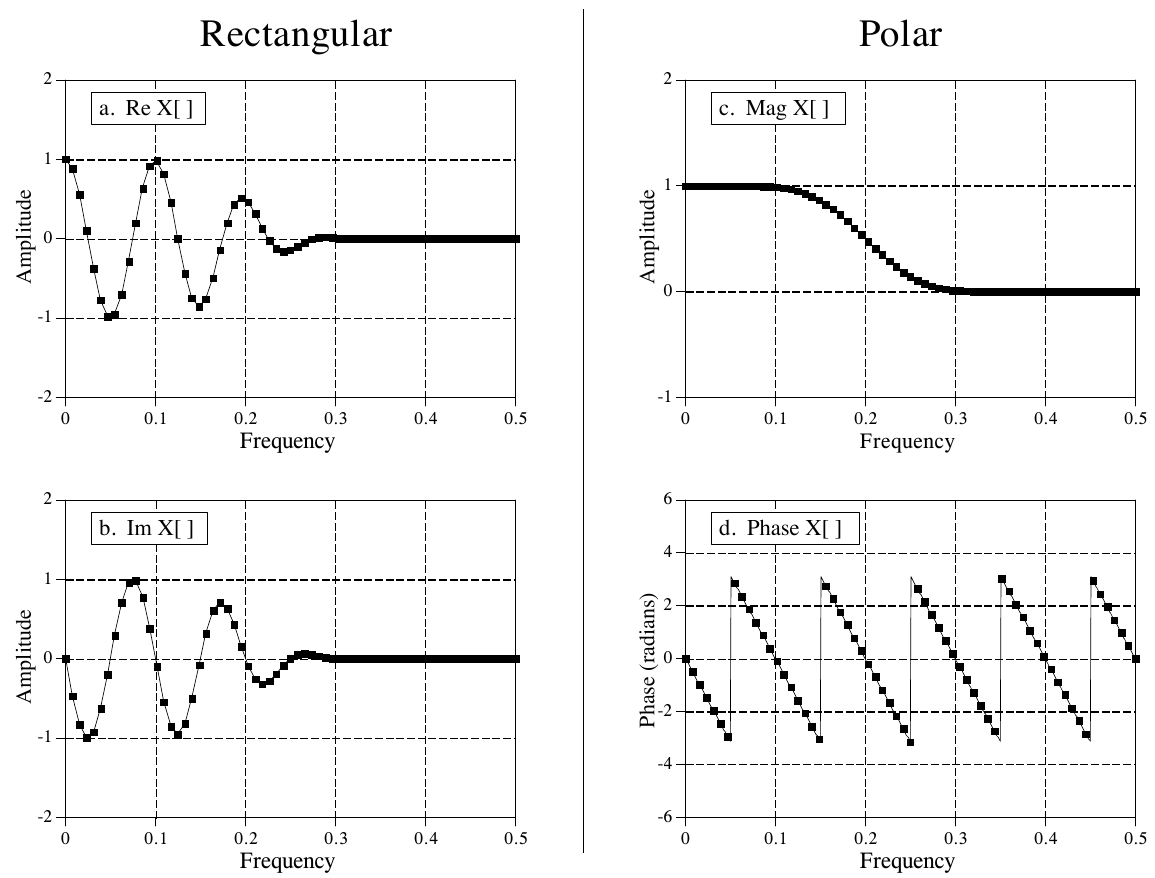
\includegraphics[width=0.963\linewidth,height=0.8\textheight,keepaspectratio]{assets/ch08/fig8-10.png}
\caption*{\textbf{图 8-10　直角坐标和极坐标频域的例子。}
本例把一个频域分别用直角坐标和极坐标表示出来。和本例一样，极坐标表示通常能让人更好地理解信号的特性。相比之下，需要做数学计算时几乎总是用直角坐标形式。特别注意，相位的第一个和最后一个采样必须为零，就像虚部一样。
（Rectangular = 直角坐标，Polar = 极坐标，Amplitude = 幅度，Phase
(radians) = 相位（弧度），Frequency = 频率。）}
\end{figure}

什么时候该用直角坐标，什么时候该用极坐标？直角坐标通常是计算（比如方程和计算机程序）的最佳选择。相比之下，图几乎总是画成极坐标形式。前面的例子表明，人几乎不可能通过看实部和虚部来理解一个频域信号的特性。在典型的程序里，频域信号一直保持直角坐标形式，直到需要给人看的时候，才做一次直角坐标到极坐标的转换。

为什么用极坐标更容易理解频域？这个问题触及了''为什么把信号分解成正弦波有用''的核心。回忆第
5
章讲的正弦保真性：正弦波进入线性系统，输出也是正弦波，并且频率和输入完全相同。只有幅度和相位会变。极坐标表示直接用各分量余弦波的幅度和相位来表示信号。相应地，系统也可以用它怎样改变每个余弦波的幅度和相位来表示。

现在想想如果在这个场景中用直角坐标会怎样。一组余弦波和正弦波的混合进入线性系统，从系统出来的也是余弦波和正弦波的混合。问题是，输入的一个余弦波可能在输出端产生余弦波和正弦波。同样，输入的一个正弦波也可能在输出端产生余弦波和正弦波。这些交叉项虽然可以理清，但整个方法和我们当初想用正弦波的初衷不相符。

\section{极坐标表示的麻烦之处}

使用极坐标表示有许多麻烦之处。没有哪个是过不去的坎，只是真的很烦人！表
8-3
是一个在直角坐标和极坐标之间转换的计算机程序，其中给出了对付其中几个麻烦的办法。

\textbf{表 8-3}（注释已译成中文）

\begin{Shaded}
\begin{Highlighting}[]
\NormalTok{100 \textquotesingle{}RECTANGULAR{-}TO{-}POLAR \& POLAR{-}TO{-}RECTANGULAR CONVERSION}
\NormalTok{110 \textquotesingle{}}
\NormalTok{120 DIM REX[256]             \textquotesingle{}REX[ ]   存放实部}
\NormalTok{130 DIM IMX[256]             \textquotesingle{}IMX[ ]   存放虚部}
\NormalTok{140 DIM MAG[256]             \textquotesingle{}MAG[ ]   存放幅值}
\NormalTok{150 DIM PHASE[256]           \textquotesingle{}PHASE[ ] 存放相位}
\NormalTok{160 \textquotesingle{}}
\NormalTok{170 PI = 3.14159265}
\NormalTok{180 \textquotesingle{}}
\NormalTok{190 GOSUB XXXX               \textquotesingle{}虚构的子程序，把数据载入 REX[ ] 和 IMX[ ]}
\NormalTok{200 \textquotesingle{}}
\NormalTok{210 \textquotesingle{}}
\NormalTok{220 \textquotesingle{}                        \textquotesingle{}直角坐标到极坐标的转换，公式 8{-}6}
\NormalTok{230 FOR K\% = 0 TO 256}
\NormalTok{240 MAG[K\%] = SQR( REX[K\%]\^{}2 + IMX[K\%]\^{}2 )                \textquotesingle{}来自公式 8{-}6}
\NormalTok{250 IF REX[K\%] = 0 THEN REX[K\%] = 1E{-}20                   \textquotesingle{}防止除以 0（麻烦 2）}
\NormalTok{260 PHASE[K\%] = ATN( IMX[K\%] / REX[K\%] )                  \textquotesingle{}来自公式 8{-}6}
\NormalTok{270 \textquotesingle{}                                                     \textquotesingle{}修正反正切（麻烦 3）}
\NormalTok{280 IF REX[K\%] \textless{} 0 AND IMX[K\%] \textless{} 0 THEN PHASE[K\%] = PHASE[K\%] {-} PI}
\NormalTok{290 IF REX[K\%] \textless{} 0 AND IMX[K\%] \textgreater{}= 0 THEN PHASE[K\%] = PHASE[K\%] + PI}
\NormalTok{300 NEXT K\%}
\NormalTok{310 \textquotesingle{}}
\NormalTok{320 \textquotesingle{}}
\NormalTok{330 \textquotesingle{}                        \textquotesingle{}极坐标到直角坐标的转换，公式 8{-}7}
\NormalTok{340 FOR K\% = 0 TO 256}
\NormalTok{350 REX[K\%] = MAG[K\%] * COS( PHASE[K\%] )}
\NormalTok{360 IMX[K\%] = MAG[K\%] * SIN( PHASE[K\%] )}
\NormalTok{370 NEXT K\%}
\NormalTok{380 \textquotesingle{}}
\NormalTok{390 END}
\end{Highlighting}
\end{Shaded}

\textbf{C 实现}（完整可编译版本见
\texttt{c/table8-3\_rect\_polar.c}。程序载入书中讨论过的几个典型点，包括
Re = 1、Im = 1 和 Re = −1、Im = −1，以及实部为 0
的点，再加一批随机点；相位与 C 标准库的 \texttt{atan2()}
对照，并检查转过去再转回来能否还原）：

\begin{Shaded}
\begin{Highlighting}[]
\PreprocessorTok{\#define NF }\DecValTok{257}\PreprocessorTok{                  }\CommentTok{/* 120～150 DIM REX[256] 等：频域 257 点 */}

\CommentTok{/* 直角 → 极坐标（公式 8{-}6），rex[] 可能被改成 1e{-}20，与原书一致 */}
\DataTypeTok{static} \DataTypeTok{void}\NormalTok{ rect\_to\_polar}\OperatorTok{(}\DataTypeTok{double} \OperatorTok{*}\NormalTok{rex}\OperatorTok{,} \DataTypeTok{const} \DataTypeTok{double} \OperatorTok{*}\NormalTok{imx}\OperatorTok{,} \DataTypeTok{double} \OperatorTok{*}\NormalTok{mag}\OperatorTok{,} \DataTypeTok{double} \OperatorTok{*}\NormalTok{phase}\OperatorTok{)}
\OperatorTok{\{}
    \ControlFlowTok{for} \OperatorTok{(}\DataTypeTok{int}\NormalTok{ k }\OperatorTok{=} \DecValTok{0}\OperatorTok{;}\NormalTok{ k }\OperatorTok{\textless{}}\NormalTok{ NF}\OperatorTok{;}\NormalTok{ k}\OperatorTok{++)} \OperatorTok{\{}          \CommentTok{/* 230 */}
\NormalTok{        mag}\OperatorTok{[}\NormalTok{k}\OperatorTok{]} \OperatorTok{=}\NormalTok{ sqrt}\OperatorTok{(}\NormalTok{rex}\OperatorTok{[}\NormalTok{k}\OperatorTok{]} \OperatorTok{*}\NormalTok{ rex}\OperatorTok{[}\NormalTok{k}\OperatorTok{]} \OperatorTok{+}\NormalTok{ imx}\OperatorTok{[}\NormalTok{k}\OperatorTok{]} \OperatorTok{*}\NormalTok{ imx}\OperatorTok{[}\NormalTok{k}\OperatorTok{]);}   \CommentTok{/* 240 */}
        \ControlFlowTok{if} \OperatorTok{(}\NormalTok{rex}\OperatorTok{[}\NormalTok{k}\OperatorTok{]} \OperatorTok{==} \DecValTok{0}\OperatorTok{)}\NormalTok{ rex}\OperatorTok{[}\NormalTok{k}\OperatorTok{]} \OperatorTok{=} \FloatTok{1e{-}20}\OperatorTok{;}    \CommentTok{/* 250：防止除零（麻烦 2） */}
\NormalTok{        phase}\OperatorTok{[}\NormalTok{k}\OperatorTok{]} \OperatorTok{=}\NormalTok{ atan}\OperatorTok{(}\NormalTok{imx}\OperatorTok{[}\NormalTok{k}\OperatorTok{]} \OperatorTok{/}\NormalTok{ rex}\OperatorTok{[}\NormalTok{k}\OperatorTok{]);}   \CommentTok{/* 260 */}
        \CommentTok{/* 270～290：修正反正切（麻烦 3），实部为负时补 ±π */}
        \ControlFlowTok{if} \OperatorTok{(}\NormalTok{rex}\OperatorTok{[}\NormalTok{k}\OperatorTok{]} \OperatorTok{\textless{}} \DecValTok{0} \OperatorTok{\&\&}\NormalTok{ imx}\OperatorTok{[}\NormalTok{k}\OperatorTok{]} \OperatorTok{\textless{}} \DecValTok{0}\OperatorTok{)}\NormalTok{  phase}\OperatorTok{[}\NormalTok{k}\OperatorTok{]} \OperatorTok{=}\NormalTok{ phase}\OperatorTok{[}\NormalTok{k}\OperatorTok{]} \OperatorTok{{-}}\NormalTok{ PI}\OperatorTok{;}  \CommentTok{/* 280 */}
        \ControlFlowTok{if} \OperatorTok{(}\NormalTok{rex}\OperatorTok{[}\NormalTok{k}\OperatorTok{]} \OperatorTok{\textless{}} \DecValTok{0} \OperatorTok{\&\&}\NormalTok{ imx}\OperatorTok{[}\NormalTok{k}\OperatorTok{]} \OperatorTok{\textgreater{}=} \DecValTok{0}\OperatorTok{)}\NormalTok{ phase}\OperatorTok{[}\NormalTok{k}\OperatorTok{]} \OperatorTok{=}\NormalTok{ phase}\OperatorTok{[}\NormalTok{k}\OperatorTok{]} \OperatorTok{+}\NormalTok{ PI}\OperatorTok{;}  \CommentTok{/* 290 */}
    \OperatorTok{\}}
\OperatorTok{\}}

\CommentTok{/* 极 → 直角坐标（公式 8{-}7） */}
\DataTypeTok{static} \DataTypeTok{void}\NormalTok{ polar\_to\_rect}\OperatorTok{(}\DataTypeTok{const} \DataTypeTok{double} \OperatorTok{*}\NormalTok{mag}\OperatorTok{,} \DataTypeTok{const} \DataTypeTok{double} \OperatorTok{*}\NormalTok{phase}\OperatorTok{,} \DataTypeTok{double} \OperatorTok{*}\NormalTok{rex}\OperatorTok{,} \DataTypeTok{double} \OperatorTok{*}\NormalTok{imx}\OperatorTok{)}
\OperatorTok{\{}
    \ControlFlowTok{for} \OperatorTok{(}\DataTypeTok{int}\NormalTok{ k }\OperatorTok{=} \DecValTok{0}\OperatorTok{;}\NormalTok{ k }\OperatorTok{\textless{}}\NormalTok{ NF}\OperatorTok{;}\NormalTok{ k}\OperatorTok{++)} \OperatorTok{\{}          \CommentTok{/* 340 */}
\NormalTok{        rex}\OperatorTok{[}\NormalTok{k}\OperatorTok{]} \OperatorTok{=}\NormalTok{ mag}\OperatorTok{[}\NormalTok{k}\OperatorTok{]} \OperatorTok{*}\NormalTok{ cos}\OperatorTok{(}\NormalTok{phase}\OperatorTok{[}\NormalTok{k}\OperatorTok{]);}    \CommentTok{/* 350 */}
\NormalTok{        imx}\OperatorTok{[}\NormalTok{k}\OperatorTok{]} \OperatorTok{=}\NormalTok{ mag}\OperatorTok{[}\NormalTok{k}\OperatorTok{]} \OperatorTok{*}\NormalTok{ sin}\OperatorTok{(}\NormalTok{phase}\OperatorTok{[}\NormalTok{k}\OperatorTok{]);}    \CommentTok{/* 360 */}
    \OperatorTok{\}}
\OperatorTok{\}}
\end{Highlighting}
\end{Shaded}

运行结果：(1, 1) \dspsym{→} 45°，(−1, −1) \dspsym{→} −135°，(−1, 1)
\dspsym{→} 135°，(0, 2) \dspsym{→} 90°，(0, −2) \dspsym{→} −90°，(−3, 0)
\dspsym{→} 180°，与 \texttt{atan2()} 完全一致；257 个点的相位与
\texttt{atan2()} 的最大差约 4e−16 弧度，直角 \dspsym{→} 极 \dspsym{→}
直角往返的最大误差约 9e−16。顺带一提，C 语言里直接用
\texttt{atan2(Im,\ Re)} 就能一次处理掉麻烦 2 和麻烦 3。

\textbf{麻烦 1：弧度还是角度}

相位可以用角度(degrees)表示，也可以用弧度(radians)表示。用角度时，相位信号的值在
−180 到 180 之间。用弧度时，每个值在 −π 到 π 之间，即 −3.141592 到
3.141592。大多数计算机语言的三角函数（余弦、正弦、反正切等）都要求用弧度。和这些长长的小数打交道很烦人，得到的数据也不好解读。例如，如果你想给信号加上
90 度相移，就得给相位加
1.570796。在程序里敲这个数要不了你的命，但确实很烦。处理这个问题最好的办法是在程序开头定义常数
PI = 3.141592，这样 90 度相移就可以写成 PI/2。角度和弧度在 DSP
中都很常用，两样你都得习惯。

\textbf{麻烦 2：除以零错误}

把直角坐标转换成极坐标时，经常会遇到实部为零、虚部不为零的频率。这只是说明相位恰好是
90 度或 −90 度。可你试试跟计算机说这个！程序用
\(\mathrm{Phase}\,X[k] = \arctan(\mathrm{Im}\,X[k]/\mathrm{Re}\,X[k])\)
计算相位时，会发生除以零错误。即使程序没有因此停止，这个频率得到的相位也不对。要避免这个问题，必须在做除法前检查实部是否为零。如果是零，就要检查虚部是正还是负，分别把相位设为
π/2 或
−π/2。最后，还得绕过这次除法。这些步骤都不难，只是可能让人恼火。表 8-3
第 250
行给出了另一种处理办法：如果实部为零，就把它改成一个小到可以忽略的数，让数学运算器在做除法时不出错。

\textbf{麻烦 3：反正切算错}

考虑一个频域采样，Re X{[}k{]} = 1，Im X{[}k{]} = 1。公式 8-6
给出对应的极坐标值 Mag X{[}k{]} = 1.414，Phase X{[}k{]} =
45°。再考虑另一个采样，Re X{[}k{]} = −1，Im X{[}k{]} = −1。公式 8-6
给出的仍然是 Mag X{[}k{]} = 1.414，Phase X{[}k{]} =
45°。问题是，这个相位是错的！它应该是
−135°。只要实部为负，就会出这个错。纠正的办法是在算出相位之后检查实部和虚部。如果实部和虚部都为负，就从算出的相位中减去
180°（即 π 弧度）。如果实部为负、虚部为正，就加上 180°（即 π 弧度）。表
8-3 程序的第 280 和 290 行展示了怎样做。（译注：原书这里写的是''第 340
和 350 行''，但那两行是极坐标到直角坐标的转换，做修正的是第 280 和 290
行。）如果你没注意到这个问题，算出的相位就只会在 −π/2 到 π/2
之间，而不是在 −π 到 π 之间。把这一点牢牢记住。如果你看到相位只延伸到
±1.5708，那就是你忘了纠正反正切计算中的歧义。

\textbf{麻烦 4：极小幅值的相位}

设想下面这个场景。你正埋头做某个 DSP
任务，突然发现相位有一部分看起来不对劲。它可能有噪声，可能乱跳，也可能干脆就是错的。你花了一个小时翻看几百行代码，终于找到了答案：对应的幅值太小，被淹没在舍入噪声(round-off
noise)里了。如果幅值小到可以忽略，相位就没有任何意义，可能取到奇怪的值。图
8-11
就是一个例子。幅度信号淹没在噪声里时，通常一眼就能看出来；那些值小得让你不得不怀疑它们没有意义。相位就不一样了。极坐标信号被噪声污染时，相位的值是
−π 到 π
之间的随机数。不幸的是，这往往看起来像个真实的信号，而不是它实际上的无意义数据。

\begin{figure}[htbp]
\centering
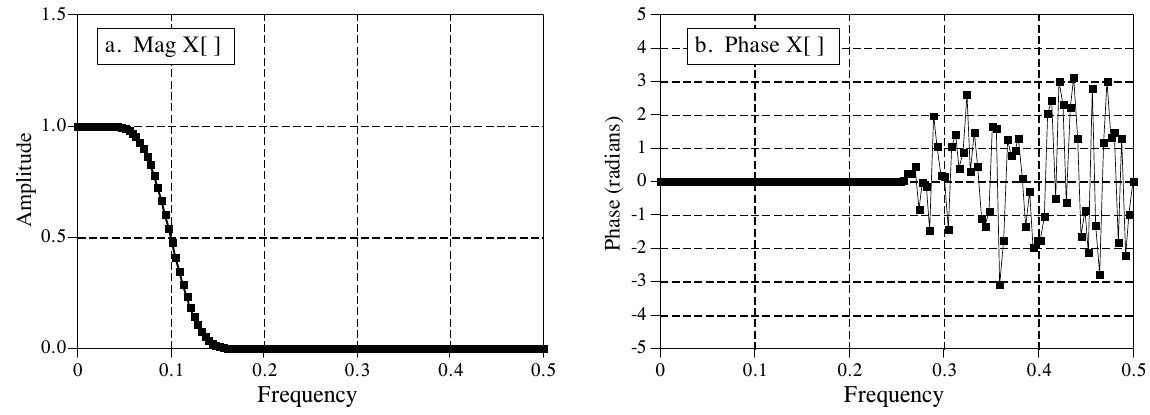
\includegraphics[width=0.958\linewidth,height=0.8\textheight,keepaspectratio]{assets/ch08/fig8-11.png}
\caption*{\textbf{图 8-11　小幅值信号的相位。}
在幅值降到很低的频率处，舍入噪声会让相位大幅乱跳。别误以为这是一个有意义的信号。
（Amplitude = 幅度，Phase (radians) = 相位（弧度），Frequency = 频率。）}
\end{figure}

\textbf{麻烦 5：相位的 2π 歧义}

再看一看图 8-10d，注意数据中的几处不连续。每当一个点看起来要降到
−3.141592 以下时，它就跳回到 3.141592。（译注：原书这里把前一个数印成了
−3.14592。）这是正弦波周期性造成的。例如，相移 θ 和相移 θ + 2π、θ +
4π、θ + 6π 等等完全一样。给相位加上 2π
的任意整数倍，任何正弦波都不变。信号中这些表面上的不连续，是计算机算法从无穷多个等价的可能中挑了它喜欢的那个的结果。它总是选最小的那个值，让相位保持在
−π 到 π 之间。

如果相位没有这些不连续，通常更容易理解，即使这意味着相位会超过 π 或低于
−π。这叫相位展开(unwrapping the phase)，图 8-12 是一个例子。如表 8-4
的程序所示，给相位的每个值加上或减去 2π
的某个整数倍。具体的值由一个让相邻采样之差最小的算法决定。

\begin{figure}[htbp]
\centering
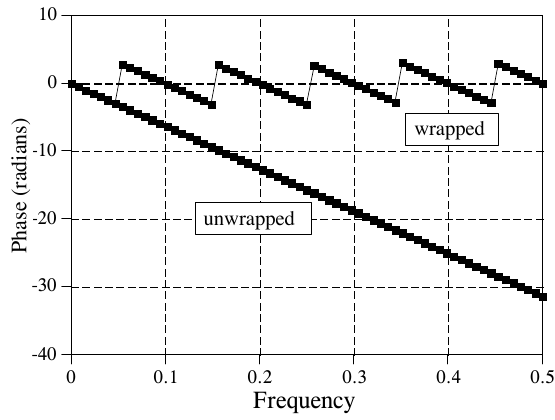
\includegraphics[width=0.463\linewidth,height=0.8\textheight,keepaspectratio]{assets/ch08/fig8-12.png}
\caption*{\textbf{图 8-12　相位展开的例子。}
上面的曲线是直角坐标到极坐标转换程序得到的典型相位信号。信号中的每个值都必须在
−π 和 π 之间（即 −3.14159 和
3.14159）。如下面的曲线所示，可以给每个采样加上或减去 2π
的整数倍来展开相位，整数的选取要让点与点之间的不连续最小。 （Phase
(radians) = 相位（弧度），Frequency = 频率，wrapped =
卷绕的（未展开），unwrapped = 展开后的。）}
\end{figure}

\textbf{表 8-4}（注释已译成中文）

\begin{Shaded}
\begin{Highlighting}[]
\NormalTok{100 \textquotesingle{} PHASE UNWRAPPING}
\NormalTok{110 \textquotesingle{}}
\NormalTok{120 DIM PHASE[256]         \textquotesingle{}PHASE[ ] 存放原始相位}
\NormalTok{130 DIM UWPHASE[256]       \textquotesingle{}UWPHASE[ ] 存放展开后的相位}
\NormalTok{140 \textquotesingle{}}
\NormalTok{150 PI = 3.14159265}
\NormalTok{160 \textquotesingle{}}
\NormalTok{170 GOSUB XXXX             \textquotesingle{}虚构的子程序，把数据载入 PHASE[ ]}
\NormalTok{180 \textquotesingle{}}
\NormalTok{190 UWPHASE[0] = 0         \textquotesingle{}所有相位信号的第一个点都是零}
\NormalTok{200 \textquotesingle{}}
\NormalTok{210 \textquotesingle{}                      \textquotesingle{}执行展开算法}
\NormalTok{220 FOR K\% = 1 TO 256}
\NormalTok{230 C\% = CINT( (UWPHASE[K\%{-}1] {-} PHASE[K\%]) / (2 * PI) )}
\NormalTok{240 UWPHASE[K\%] = PHASE[K\%] + C\%*2*PI}
\NormalTok{250 NEXT K\%}
\NormalTok{260 \textquotesingle{}}
\NormalTok{270 END}
\end{Highlighting}
\end{Shaded}

\textbf{C 实现}（完整可编译版本见
\texttt{c/table8-4\_phase\_unwrap.c}。程序按图 8-12
的样子生成数据：一条从 0 线性降到 −10π（约 −31.4）的真实相位，相当于延迟
10 个采样点；把它折回 −π～π 作为输入，展开后与真实相位对照）：

\begin{Shaded}
\begin{Highlighting}[]
\PreprocessorTok{\#define NF }\DecValTok{257}\PreprocessorTok{                  }\CommentTok{/* 120～130 DIM PHASE[256]、UWPHASE[256] */}

\NormalTok{    uwphase}\OperatorTok{[}\DecValTok{0}\OperatorTok{]} \OperatorTok{=} \DecValTok{0}\OperatorTok{;}                         \CommentTok{/* 190：所有相位信号的第一点都是 0 */}
    \ControlFlowTok{for} \OperatorTok{(}\DataTypeTok{int}\NormalTok{ k }\OperatorTok{=} \DecValTok{1}\OperatorTok{;}\NormalTok{ k }\OperatorTok{\textless{}}\NormalTok{ NF}\OperatorTok{;}\NormalTok{ k}\OperatorTok{++)} \OperatorTok{\{}          \CommentTok{/* 220 */}
        \CommentTok{/* 230：CINT 是四舍五入取整，算出要补几个 2π */}
        \DataTypeTok{long}\NormalTok{ c }\OperatorTok{=}\NormalTok{ lround}\OperatorTok{((}\NormalTok{uwphase}\OperatorTok{[}\NormalTok{k }\OperatorTok{{-}} \DecValTok{1}\OperatorTok{]} \OperatorTok{{-}}\NormalTok{ phase}\OperatorTok{[}\NormalTok{k}\OperatorTok{])} \OperatorTok{/} \OperatorTok{(}\DecValTok{2} \OperatorTok{*}\NormalTok{ PI}\OperatorTok{));}
\NormalTok{        uwphase}\OperatorTok{[}\NormalTok{k}\OperatorTok{]} \OperatorTok{=}\NormalTok{ phase}\OperatorTok{[}\NormalTok{k}\OperatorTok{]} \OperatorTok{+}\NormalTok{ c }\OperatorTok{*} \DecValTok{2} \OperatorTok{*}\NormalTok{ PI}\OperatorTok{;} \CommentTok{/* 240 */}
    \OperatorTok{\}}
\end{Highlighting}
\end{Shaded}

运行结果：展开后最后一点（频率 0.5）为 −31.4159，与真实值 −10π
一致；全部 257 点与真实相位的最大误差约 2e−15。

\textbf{麻烦 6：幅值总是正的（相位的 π 歧义）}

图 8-13
用直角坐标和极坐标两种形式画出了一个频域信号。实部平滑，很容易理解，虚部则全为零。相比之下，极坐标信号里有突然的不连续和尖角。这是因为按定义，幅值必须总是正的。每当实部降到零以下，幅值就通过把相位改变
π（或
−π，两者是一回事）来保持为正。这对数学来说不是问题，但不规则的曲线可能很难解读。

\begin{figure}[htbp]
\centering
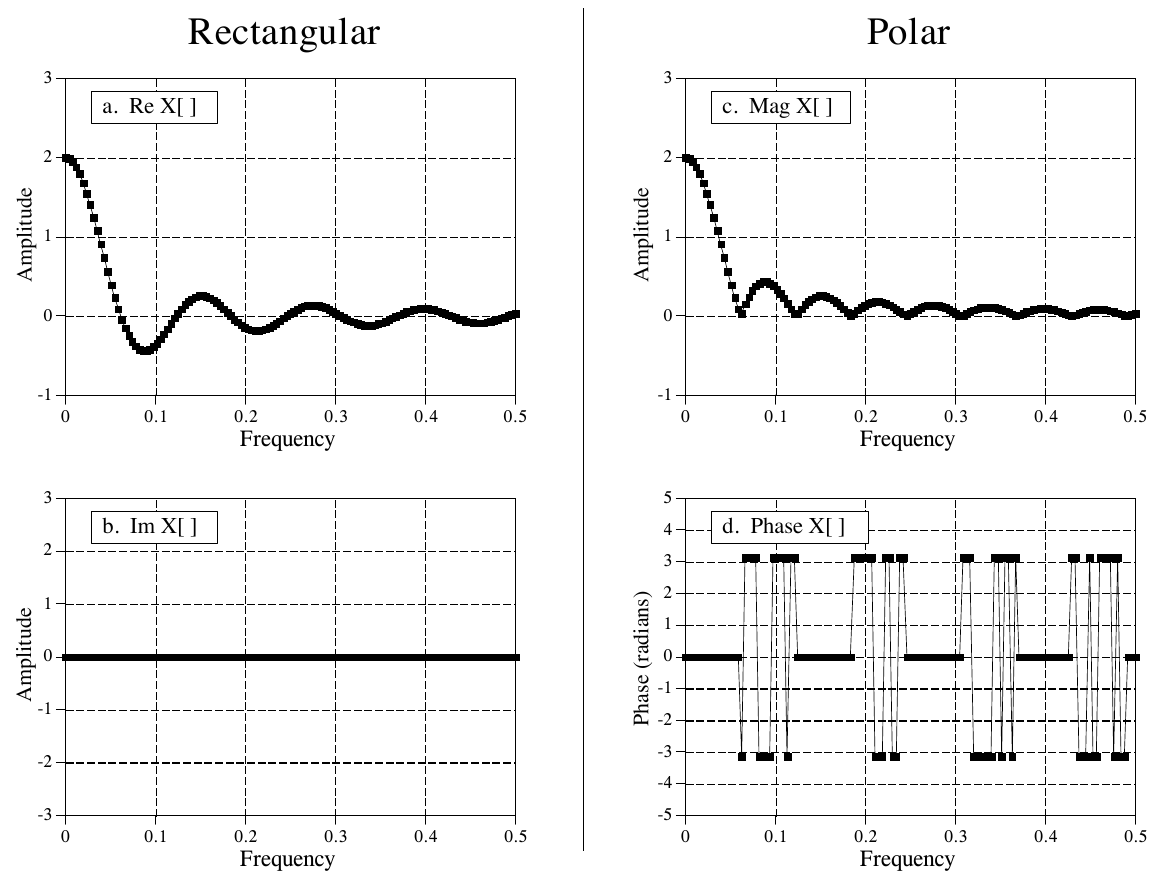
\includegraphics[width=0.963\linewidth,height=0.8\textheight,keepaspectratio]{assets/ch08/fig8-13.png}
\caption*{\textbf{图 8-13　直角坐标和极坐标形式的示例信号。}
由于幅值（按定义）必须总是正的，幅值和相位可能出现突然的不连续和尖角。图
(d) 还展示了另一个麻烦：随机噪声会让相位在 π 和 −π 之间快速来回跳。
（Rectangular = 直角坐标，Polar = 极坐标，Amplitude = 幅度，Phase
(radians) = 相位（弧度），Frequency = 频率。）}
\end{figure}

一个解决办法是允许幅值取负值。在图 8-13
的例子里，这会让幅值看起来和实部一样，而相位全为零。如果这有助于你理解，这样做没什么不对。只是要小心，别把带负值的信号叫做''幅值''，因为这违反了它的正式定义。本书用一个含糊其辞的说法------展开幅值(unwrapped
magnitude)------来表示允许取负值的''幅值''。

\textbf{麻烦 7：π 和 −π 之间的尖刺}

由于 π 和 −π
代表同一个相移，舍入噪声会让相位中相邻的点在这两个值之间快速来回切换。如图
8-13d
所示，这会在本来平滑的曲线上造成急剧的断点和尖刺。别被骗了，相位其实并没有这么不连续。
